\documentclass[11pt,a4paper,oneside]{report}

\usepackage[T1]{fontenc}
\usepackage[utf8]{inputenc}
\usepackage{newpxtext}
\usepackage{amsmath,amssymb,mathtools}
\usepackage{newpxmath}
\usepackage{dsfont}
\usepackage[margin=2.8cm]{geometry}
\usepackage{microtype}
\usepackage{graphicx}
\usepackage{booktabs}
\graphicspath{{figures/}}
\usepackage{float}
\usepackage{xcolor}
\usepackage[skins,breakable]{tcolorbox}
\usepackage[colorlinks=true,linkcolor=blue!50!black,citecolor=blue!50!black,urlcolor=blue!50!black]{hyperref}
\usepackage[capitalise,noabbrev]{cleveref}
\hypersetup{pdftitle={Introduction to String Theory, Part II: String compactifications},
  pdfsubject={Lecture notes on Module 1, University of Bologna, 2026/27}}

\newif\ifdarktitle \darktitletrue
\definecolor{titlebg}{HTML}{140A22}
\definecolor{titlerule}{HTML}{FF9433}
\ifdarktitle
  \definecolor{titlesub}{HTML}{DCCFEA}\newcommand{\titleart}{fig_title-art-dark}
\else
  \definecolor{titlesub}{HTML}{4A4D55}\newcommand{\titleart}{fig_title-art}
\fi

\numberwithin{equation}{chapter}
\newcommand{\lecturedate}[1]{%
  \vspace*{-1.5ex}{\noindent\large\itshape #1\par}\vspace{2ex}}

\newcommand{\dd}{\mathrm{d}}
\newcommand{\GeV}{\,\mathrm{GeV}}
\newcommand{\TeV}{\,\mathrm{TeV}}
\newcommand{\Mp}{M_{P}}
\newcommand{\Ms}{M_{s}}
\newcommand{\MKK}{M_{K\!K}}
\newcommand{\ls}{\ell_s}
\newcommand{\Vol}{\mathcal{V}}
\newcommand{\R}{\mathbb{R}}
\newcommand{\Z}{\mathbb{Z}}
\newcommand{\C}{\mathbb{C}}
\newcommand{\one}{\mathds{1}}
\newcommand{\hodge}{\mathord{\star}}
\DeclareMathOperator{\Hol}{Hol}
\DeclareMathOperator{\Tr}{Tr}
\DeclareMathOperator{\tr}{tr}


\begin{document}

\hypersetup{pageanchor=false}%
\begin{titlepage}
  \ifdarktitle
    \AddToHookNext{shipout/background}{%
      \put(0pt,-\paperheight){\textcolor{titlebg}{\rule{\paperwidth}{\paperheight}}}}%
    \color{white}%
  \fi
  \centering
  \vspace*{\stretch{1}}
  \includegraphics[width=0.74\textwidth]{\titleart}
  \vspace{5ex}
  {\Huge\bfseries Introduction to String Theory\par}
  \vspace{2ex}
  {\color{titlerule}\rule{0.18\textwidth}{0.8pt}\par}
  \vspace{2ex}
  {\LARGE\color{titlesub} Part II: String compactifications\par}
  \vspace{4ex}
  {\large\color{titlesub} Lecture notes on Module 1\par}
  \vspace{1ex}
  {\large\color{titlesub} University of Bologna, academic year 2026/27\par}
  \vspace*{\stretch{1.6}}
\end{titlepage}
\hypersetup{pageanchor=true}

\chapter*{Editor's note}

{\itshape\setlength{\parskip}{1.2ex}\setlength{\parindent}{0pt}%
These are notes for Module 1 of the ``Introduction to String Theory’’ course at the University of Bologna. Apart from this page,
they were written entirely by Claude Opus 5.5 from scans of handwritten lecture notes taken by me and other students in 2026.
They are an independent reconstruction, not a record of the lectures.
The lecturer has neither seen nor endorsed them, and they may depart from the lectures in content, emphasis and conventions.
Any errors are mine (and Claude’s).

I hope these notes prove useful, although I doubt they will hold much value in the years to come, when far more powerful
models will be available.

This leads me to some (somewhat uncalled-for and unprofessional) reflections on the strange times
I am living through. I remember the moment, a few years ago, when a new OpenAI model turned out to be a better coder than me.
Given how fast these models were improving, I knew I would never catch up.
Now I feel the same way about physics. I find it hard to believe that I will ever solve a physics problem that an AI
could not solve faster and more cheaply. This has made me genuinely sad for months now.

But, to complicate matters, mixed in with that sadness is real excitement. What will these systems teach us
about the deepest mysteries in physics? About quantum gravity and string theory? Which problems
will they solve? Perhaps the most important practical question a young graduate student can now ask is: ``How can I
position myself to understand the output of the equivalent of a thousand Wittens, working nonstop at fifty times human speed?''
I hope these lecture notes can help with that task.
 \par}

\par\bigskip
\begin{flushright}
  \textit{LazyLagrangian}\\
  \textit{6 November 2026}
\end{flushright}


\tableofcontents

\chapter*{Notation and conventions}
\addcontentsline{toc}{chapter}{Notation and conventions}

This chapter fixes one set of conventions for the whole of the notes. They are the ones most common in the string-compactification literature, which are not always those used on the board; where a lecture writes a formula in another convention, it is converted to the one below.

\paragraph{Units and approximate equalities.} We use natural units, $\hbar = c = 1$, so that masses, energies and inverse lengths are measured in $\mathrm{GeV}$. An equality sign is exact. The sign ``$\simeq$'' means equality up to numerical factors of order one (such as $2$, $\pi$ or $\sqrt{4\pi}$) that are dropped when only the parametric dependence on $g_s$ and $\Vol$ matters, and ``$\sim$'' means ``of the order of''. When a relation is first derived its factors are kept, and it is then quoted with ``$\simeq$''.

\paragraph{Metric and curvature.} Metrics have mostly-plus signature, $\eta_{MN} = \mathrm{diag}(-1,+1,\dots,+1)$, as in Polchinski~\cite{Polchinski}, Tong~\cite{Tong}, Wess and Bagger, and most of the compactification literature. The Riemann tensor is $R^\rho{}_{\sigma\mu\nu} = \partial_\mu\Gamma^\rho_{\nu\sigma} - \partial_\nu\Gamma^\rho_{\mu\sigma} + \Gamma^\rho_{\mu\lambda}\Gamma^\lambda_{\nu\sigma} - \Gamma^\rho_{\nu\lambda}\Gamma^\lambda_{\mu\sigma}$, the Ricci tensor is $R_{\mu\nu} = R^\rho{}_{\mu\rho\nu}$, and a sphere has positive Ricci scalar. With these choices the four-dimensional Einstein--Hilbert action is
\begin{equation*}
  S_{\mathrm{EH}} = \frac{\Mp^2}{2}\int\dd^4x\,\sqrt{-g}\,R .
\end{equation*}
For a Lorentzian metric we write $\sqrt{-g}$, for the Riemannian metric of the compact space $\sqrt{g}$.

\paragraph{Spaces, coordinates and indices.} Ten-dimensional spacetime is $X_{10} = \R^{1,3}\times Y_6$, with $Y_6$ a compact six-dimensional manifold and coordinates $X^M = (x^\mu, y^m)$.
\begin{itemize}
  \item Capital Latin indices $M,N,P = 0,\dots,9$ are ten-dimensional.
  \item Greek indices $\mu,\nu,\rho = 0,\dots,3$ are four-dimensional.
  \item Lower-case Latin indices $m,n,p = 4,\dots,9$ are real indices on $Y_6$.
  \item The indices $i,j = 1,2,3$ and $\bar\imath,\bar\jmath$ label holomorphic and antiholomorphic coordinates $z^i$, $\bar z^{\bar\jmath}$ on $Y_6$ when it is a complex manifold.
\end{itemize}
The ten-dimensional metric is $G_{MN}$, with determinant $G$ and Ricci scalar $R_{10}$. On a product space it splits into the four-dimensional metric $g_{\mu\nu}$ (determinant $g_4$, Ricci scalar $R_4$) and the internal metric $g_{mn}$ (determinant $g_6$, Ricci scalar $R_6$). The volume of the compact space is $\mathrm{Vol}(Y_6) = \int_{Y_6}\dd^6y\,\sqrt{g_6}$. The holonomy group of $Y_6$ is $\Hol(Y_6)$, and $\one$ is the identity.

\paragraph{String length and string scale.} The only dimensionful parameter of string theory is $\alpha'$, related to the string tension by $T = 1/(2\pi\alpha')$. Following the lecture and the moduli-stabilisation literature we define
\begin{equation*}
  \ls = 2\pi\sqrt{\alpha'} ,\qquad \Ms = \frac{1}{\ls} .
\end{equation*}
Polchinski and Tong use $\ls = \sqrt{\alpha'}$ instead, which is smaller by $2\pi$. The virtue of the factor $2\pi$ is that it absorbs the powers of $2\pi$ of the ten-dimensional gravitational coupling, $2\kappa_{10}^2 = (2\pi)^7\alpha'^4 = \ls^8/2\pi$, and of the D$p$-brane tensions, $T_p = 2\pi\Ms^{p+1}/g_s$. The price is that T-duality, which exchanges a circle of radius $R$ with one of radius $\alpha'/R$, reads $R\to\alpha'/R = 1/(4\pi^2\Ms^2R)$ (\cref{eq:L2-Tduality}); the self-dual radius is $\sqrt{\alpha'} = \ls/2\pi$.

\paragraph{Dilaton, string coupling and frames.} The dilaton $\phi$ is a field. Its vacuum expectation value is $\phi_0 \equiv \langle\phi\rangle$, and the string coupling is
\begin{equation*}
  g_s = e^{\phi_0} .
\end{equation*}
The \emph{string frame} metric $G_{MN}$ is the one to which the string couples on the worldsheet; in it the gravitational action carries a factor $e^{-2\phi}$ in front of the Ricci scalar (\cref{eq:L1-S10}). The ten-dimensional \emph{Einstein frame} metric is
\begin{equation*}
  G^E_{MN} = e^{-(\phi-\phi_0)/2}\,G_{MN} ,
\end{equation*}
in which the gravitational action takes the Einstein--Hilbert form $\frac{1}{2\kappa_{10}^2 g_s^2}\int\dd^{10}X\sqrt{-G_E}\,R_{10}[G_E]$. Because $\phi_0$ is subtracted, the two frames coincide in a vacuum with constant dilaton, $\phi = \phi_0$. In particular a volume measured in string units is the same number in both frames, and the relations between scales derived in \cref{ch:L1}, $\Mp^2 = 4\pi\Vol\Ms^2/g_s^2$ and $\MKK \simeq \Ms/\Vol^{1/6}$, hold in either.

Much of the moduli-stabilisation literature uses instead $G^E_{MN} = e^{-\phi/2}G_{MN}$, without the subtraction. In a vacuum the two Einstein frames then differ by the constant factor $g_s^{-1/2}$, so that a dimensionless volume in that convention is $\Vol' = g_s^{-3/2}\,\Vol$, and the same relations read $\Ms = g_s^{1/4}\Mp/\sqrt{4\pi\Vol'}$ and $\MKK\simeq\Mp/(\sqrt{4\pi}\,\Vol'^{2/3})$. Formulas taken from such references are converted with $\Vol' = g_s^{-3/2}\Vol$.

\paragraph{Volume.} $\Vol$ is the dimensionless volume of $Y_6$ in units of $\ls^6$, measured with the Einstein-frame metric:
\begin{equation*}
  \mathrm{Vol}(Y_6) = \Vol\,\ls^6 .
\end{equation*}

\paragraph{Planck mass.} $\Mp$ is the reduced Planck mass,
\begin{equation*}
  \Mp = (8\pi G_N)^{-1/2} \simeq 2.4\times10^{18}\GeV ,
\end{equation*}
the coefficient of the four-dimensional Einstein--Hilbert action above. Four-dimensional actions are written in the four-dimensional Einstein frame, in which this coefficient is constant.

\paragraph{Counting supersymmetries.} $\mathcal N$ counts supersymmetry generators in units of the smallest spinor of the spacetime dimension. In ten dimensions this is a Majorana--Weyl spinor, with $16$ real components, so type IIA and IIB supergravity, with two of them, have ten-dimensional $\mathcal N=2$ and $32$ real supercharges. The two have opposite chirality in type IIA, and the same chirality in type IIB, which is therefore chiral. In four dimensions the unit is a Majorana spinor, equivalently a Weyl spinor and its conjugate, with $4$ real components, so that four-dimensional $\mathcal N = 8,4,2,1$ correspond to $32,16,8,4$ real supercharges. A subscript $\pm$ on a ten-dimensional spinor, as in $\psi_{M+}$ or $\lambda_-$, gives its chirality, the eigenvalue $\pm1$ of $\Gamma_{11} = \Gamma^0\Gamma^1\cdots\Gamma^9$, which squares to one in our signature.

\paragraph{Forms.} A $p$-form $C_p = \frac{1}{p!}C_{M_1\dots M_p}\,\dd X^{M_1}\wedge\dots\wedge\dd X^{M_p}$ is identified with its totally antisymmetric components, e.g.\ $C_2\leftrightarrow C_{MN} = C_{[MN]}$. The NS--NS two-form is $B$, with field strength $H = \dd B$; the R--R forms are $C_p$, with field strengths $F_{p+1} = \dd C_p + \dots$. A form $\omega$ on $Y_6$ is harmonic if $\Delta\omega = 0$, with $\Delta = \dd\dd^\dagger + \dd^\dagger\dd$ the Laplacian of the internal metric. On a complex manifold a $(p,q)$-form has $p$ holomorphic and $q$ antiholomorphic indices.

\paragraph{Moduli.} The Hodge numbers $h^{p,q}$ of $Y_6$ count its linearly independent harmonic $(p,q)$-forms; for a Calabi--Yau threefold the non-trivial ones are $h^{1,1}$ and $h^{2,1}$ ($=h^{1,2}$). A generic modulus is $\phi^I$; in discussing the couplings of moduli to matter, $\phi$ without index also stands for a generic canonically normalised modulus. The Kähler moduli are $T_i$, $i = 1,\dots,h^{1,1}$, and the complex-structure moduli $U_a$, $a = 1,\dots,h^{2,1}$. The index $i$ of $T_i$ is a label, not a holomorphic index; the two are never needed in the same formula, and the context tells which is meant. The axio-dilaton is
\begin{equation*}
  S = e^{-\phi} + i\,C_0 ,\qquad \langle\mathrm{Re}\,S\rangle = \frac{1}{g_s} ,
\end{equation*}
as in the lecture and in the Large Volume Scenario literature. Much of the flux-compactification literature (GKP, KKLT, F-theory) uses instead $\tau = C_0 + i\,e^{-\phi} = i\bar S$, on which the $SL(2,\Z)$ S-duality of type IIB acts by fractional linear transformations; formulas taken from there are converted with $\tau = i\bar S$. With an index, $\tau_i$ will denote the volumes of four-cycles, the real parts of the $T_i$. Gauge couplings are $\alpha = g^2/4\pi$; the hypercharge coupling is GUT-normalised, $\alpha_1 = \frac53\alpha_Y$.

\paragraph{Supergravity.} Four-dimensional $\mathcal N=1$ supergravity, with Kähler potential $K$ and superpotential $W$, is written in the conventions of Wess and Bagger.


\chapter{From ten to four dimensions: scales and supersymmetry}
\label{ch:L1}
\lecturedate{Lecture of 5 November 2026}

This first lecture of the second part of the course is an overview. Its purpose is to give a global picture of how one goes from ten-dimensional superstring theory to the four-dimensional world we observe, before the following lectures fill in the details. Two questions organise it. The first is quantitative: when six of the ten dimensions are compact, which energy scales appear, and in which window of energies can we trust which effective description? The answer is a hierarchy of three scales, the Planck mass, the string scale and the Kaluza--Klein scale, controlled by two numbers, the string coupling $g_s$ and the volume $\Vol$ of the extra dimensions in string units. The second question is qualitative: how much of the supersymmetry of ten-dimensional string theory survives in four dimensions? The answer depends on the holonomy of the compact space, and it is what singles out Calabi--Yau manifolds.

\section{Where we stand and where we are going}
\label{sec:L1-aims}

The first part of the course, Prof.\ Ling Lin's module, described the string from the point of view of its worldsheet. The fundamental object is a vibrating string, and quantising it means quantising the two-dimensional field theory that lives on the surface it sweeps out, the worldsheet, whose fields are the spacetime coordinates $X^M$ of the string. This is a two-dimensional conformal field theory. It has a Weyl symmetry, and the requirement that this symmetry has no anomaly fixes the dimension of spacetime, $D = 26$ for the bosonic string. The spectrum of the bosonic string contains a tachyon, a sign that the theory is unstable. To get rid of it one adds fermions on the worldsheet. The result is the superstring, whose critical dimension is $D=10$. The Gliozzi--Scherk--Olive (GSO) projection removes the tachyon, and the theory turns out to be supersymmetric not only on the worldsheet but also in spacetime. The quantum states of the string form a tower of modes, a few of them massless and the others massive, and each of them corresponds to a spacetime field; among the massless modes of the closed string are the metric $G_{MN}$, the Kalb--Ramond two-form $B_{MN}$ and the dilaton $\phi$.

Besides closed strings there are open strings, whose endpoints are attached to extended objects, the D$p$-branes, of any dimension up to that of spacetime. The open strings ending on a brane describe fields that live on it, in particular gauge fields, and on a stack of $N$ coincident branes they give a non-abelian gauge theory with gauge group $U(N)$.
There are five consistent perturbative superstring theories, which differ in how the spectrum is chosen: type I, types IIA and IIB, in which worldsheet fermions are added for both the left- and the right-moving degrees of freedom of the closed string, and the two heterotic theories, with gauge groups $SO(32)$ and $E_8\times E_8$, in which only the right-movers are supersymmetrised. Perturbatively they look different, but they are related by dualities, some of which exchange a strongly coupled theory with a weakly coupled one, and they are understood as different limits of a single underlying theory, M-theory (\cref{sec:L2-dualities}). Loop amplitudes are sums over Riemann surfaces of increasing genus, which replace the Feynman diagrams of field theory; since the string has a finite size, which acts as a natural cutoff, they have no ultraviolet divergences.

From here one could follow many directions: the quantum properties of each of the five theories, their mathematical structure, black holes in ten or fewer dimensions. This part of the course follows one of them, \emph{string compactifications}: how to reproduce our four-dimensional world, with the Standard Model and cosmology, starting from ten-dimensional string theory. The idea is to take spacetime to be four-dimensional Minkowski space times a compact six-dimensional space, and to go to energies below the inverse size of the extra dimensions, where they can no longer be seen. What remains is a four-dimensional effective theory with local supersymmetry, a supergravity theory of the kind met in the supersymmetry course, with the important difference that it is not written down by hand: it is derived from a consistent theory of quantum gravity. Its physics depends strongly on the geometry and the topology of the extra dimensions, so we shall need some differential geometry and Calabi--Yau manifolds, and D-branes will play an essential role in reproducing the non-abelian gauge theories seen in nature. The module covers the low-energy effective action of string theory, D-brane actions and dualities, type II compactifications on Calabi--Yau manifolds, flux compactifications and moduli stabilisation, supersymmetry breaking in string models, and the basic principles of string cosmology.

We shall see that the way down from ten to four dimensions is not unique. There is a \emph{landscape}, or a multiverse, of solutions, each corresponding to a different four-dimensional universe. The goal is to find at least one that reproduces what we know, the Standard Model and cosmology, and possibly also offers solutions to the open problems recalled at the beginning of the supersymmetry course: inflation, dark matter, dark energy, the hierarchy problem and supersymmetry breaking.

The subject is vast, and this part of the course is necessarily dense. Rather than deriving everything systematically from a set of assumptions, which would cover one topic in depth but give a very partial view of the subject, the aim is a global understanding of the whole picture, with details to be studied afterwards where one is interested. The first lectures are therefore largely qualitative, meant to build intuition for how things go; later lectures return to the main steps with explicit computations, together with the mathematical background they need (differential forms, complex manifolds, branes and the dualities that generalise electric--magnetic duality).

\paragraph{References.} The following books, reviews and lecture notes cover the material of this part of the course, and much more:
\begin{enumerate}
  \item L.~E. Ibáñez and A.~M. Uranga, \emph{String Theory and Particle Physics: An Introduction to String Phenomenology}~\cite{IbanezUranga};
  \item A.~Hebecker, \emph{Naturalness, String Landscape and Multiverse}, lecture notes freely available online~\cite{Hebecker};
  \item R.~Blumenhagen, B.~Körs, D.~Lüst and S.~Stieberger, \emph{Four-dimensional string compactifications with D-branes, orientifolds and fluxes}, a long review~\cite{BKLS};
  \item lecture notes by J.~Louis, available on his website~\cite{Louis};
  \item D.~Baumann and L.~McAllister, \emph{Inflation and String Theory}, a book whose lecture-note version is available online~\cite{BaumannMcAllister};
  \item M.~Cicoli, J.~P. Conlon, A.~Maharana, S.~Parameswaran, F.~Quevedo and I.~Zavala, \emph{String cosmology: from the early universe to today}~\cite{StringCosmoReview}.
\end{enumerate}
The first four are oriented towards particle physics and the low-energy limit of string theory. The last two are oriented towards cosmology, which is a particularly promising arena for testing string theory, because some cosmological questions, inflation above all, can only be addressed reliably in an ultraviolet-complete theory. The review~\cite{StringCosmoReview} starts with an introduction to compactifications and then follows the whole cosmological history, from inflation through reheating to dark matter and dark energy.

The exam consists of a twelve-minute slide presentation on a topic chosen by the student, from either part of the course, followed by questions on that topic. Reproducing a topic as it was presented in the lectures can earn up to 29/30; for 30 or 30 cum laude something more is expected, for which references can be asked to the lecturers. A mark can be turned down once.

\section{Superstring theory as a theory of quantum gravity}
\label{sec:L1-qg}

Superstring theory is a consistent quantum theory, and the reason for the interest in it is that it is a consistent theory of quantum \emph{gravity}. Its massless spectrum contains a symmetric tensor field $G_{MN}(X)$, the metric: there is a massless spin-two particle, the graviton, and so there is gravity, in a theory whose loop amplitudes are finite. But string theory is not only a theory of gravity. It also contains gauge interactions and matter, basically all the rest of physics, so that it is a candidate for a unified description of all interactions, and it is a framework large enough that other approaches to quantum gravity may turn out to be contained in it.

The theory is consistent because two potential problems are absent. There are no tachyons, thanks to the GSO projection, and there are no states of negative norm. The second requirement is the absence of a Weyl anomaly on the worldsheet, and it fixes the number of spacetime dimensions to the critical dimension
\begin{equation}
  D = 10 .
  \label{eq:L1-D10}
\end{equation}
String theory is the only theory we know that predicts the number of spacetime dimensions. The prediction is, at first sight, wrong, since we see four dimensions. But it is not so bad: the answer is a positive integer, and it could have been worse.

\begin{addition}
\emph{Where $D=10$ comes from.} In the covariant quantisation of the superstring the worldsheet theory contains, besides the $D$ bosons $X^M$ and their $D$ fermionic partners, the ghosts that come from fixing the worldsheet diffeomorphisms and local supersymmetry. Each field contributes to the central charge of the Virasoro algebra: $1$ for each boson, $\tfrac12$ for each Majorana fermion, $-26$ for the $bc$ ghosts and $+11$ for the $\beta\gamma$ superghosts. The Weyl anomaly is proportional to the total, $c_{\text{tot}} = \tfrac32 D - 15$, and vanishes only for $D=10$, i.e.\ for a ``matter'' theory of central charge $c = 15$. The same condition makes the BRST charge nilpotent, $Q_B^2 = 0$, which is what guarantees that the negative-norm states introduced by covariant quantisation decouple from the physical spectrum. For the bosonic string the same counting gives $D - 26 = 0$.
\end{addition}

\section{Compactification and the Kaluza--Klein scale}
\label{sec:L1-KK}

To make contact with the real world we must study \emph{string compactifications}. Ten-dimensional Minkowski space $\R^{1,9}$ is a solution of string theory, but there are others, in which ten-dimensional spacetime is the product of four-dimensional Minkowski space and a six-dimensional manifold,
\begin{equation}
  X_{10} = \R^{1,3}\times Y_6 ,
  \label{eq:L1-X10}
\end{equation}
where $Y_6$ is a \emph{compact} space: a six-sphere, a six-dimensional torus, or something more complicated. Its volume $\mathrm{Vol}(Y_6)$ has dimensions of a length to the sixth power, so its $-1/6$ power is an energy, the \emph{Kaluza--Klein scale},
\begin{equation}
  \MKK \coloneqq \frac{1}{\mathrm{Vol}(Y_6)^{1/6}} .
  \label{eq:L1-MKK-def}
\end{equation}
$\MKK$ is the energy above which one starts to see the extra dimensions; equivalently, $1/\MKK$ is the length scale below which they become visible. We expect
\begin{equation*}
  \MKK \gg E_{\mathrm{LHC}} \sim 1\TeV ,
\end{equation*}
the energies probed at the LHC, and this explains why we have not seen extra dimensions.

The idea is easiest to picture in two dimensions. Take a spacetime that is a cylinder, with one extended direction and one direction curled up into a circle, and look at it from very far away: one sees a line, not the circle (\cref{fig:L1-cylinder}). In the same way, it is not so strange to expect that at every point of our four-dimensional spacetime there is a six-dimensional curled-up space that we do not see, simply because it is too small.

\begin{figure}[tbp]
  \centering
  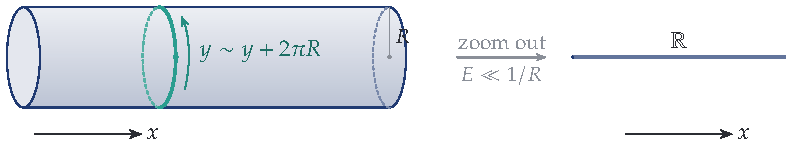
\includegraphics{fig_L1-cylinder}
  \caption{A cylinder $\R\times S^1$ seen from close by and from far away: at distances much larger than its circumference, or energies much lower than $1/R$, it looks like a line. Every point of the line carries a small circle, as every point of $\R^{1,3}$ carries a copy of $Y_6$.}\label{fig:L1-cylinder}
\end{figure}

\begin{addition}
\emph{The Kaluza--Klein tower.} The name of $\MKK$ comes from the tower of four-dimensional particles that a single higher-dimensional field gives, as met in the supersymmetry course. For a massless scalar $\Phi(x,y)$ on $\R^{1,3}\times S^1$, with $y\sim y+2\pi R$, the Fourier expansion $\Phi = \sum_{n\in\Z}\varphi_n(x)\,e^{iny/R}$ turns the five-dimensional wave equation into four-dimensional Klein--Gordon equations for the modes $\varphi_n$ with masses $m_n = |n|/R$. At energies $E\ll1/R$ only the zero mode $\varphi_0$ can be produced, and the theory looks four-dimensional. On a six-dimensional torus with six circles of radius $R$, $\mathrm{Vol}(Y_6) = (2\pi R)^6$ and the lightest massive modes have $m = 1/R = 2\pi/\mathrm{Vol}(Y_6)^{1/6}$. Thus \cref{eq:L1-MKK-def} fixes $\MKK$ only up to a factor of order one (here $2\pi$), and for a less symmetric $Y_6$ the precise spectrum depends on its shape, not only on its volume; what matters for us is the scaling with the volume.
\end{addition}

\section{The string scale and the Planck scale}
\label{sec:L1-scales}

Let us now place the relevant scales on an energy axis. Somewhere high up is the four-dimensional Planck mass $\Mp$; somewhere below it is the \emph{string scale}, the inverse of the string length,
\begin{equation}
  \Ms = \frac{1}{\ls} ,\qquad \ls = 2\pi\sqrt{\alpha'} .
  \label{eq:L1-Ms-def}
\end{equation}
The string length is set by the only free parameter of string theory, $\alpha'$, which determines the string tension, $T = 1/(2\pi\alpha')$. When the string is quantised, its vibrational modes give states that are either massless or have masses set by $1/\sqrt{\alpha'} = 2\pi\Ms$, growing with the level of excitation. Why have we drawn $\Ms$ below $\Mp$? To answer this, we have to relate the two.

\subsection{The ten-dimensional action and the dilaton}

From the scattering amplitudes of strings, at tree level and at loop level, one can reconstruct the effective action of the massless modes of the string in ten dimensions. Among its terms is the ten-dimensional Einstein--Hilbert term
\begin{equation}
  S_{10} \supset \frac{1}{2\kappa_{10}^2}\int\dd^{10}X\,\sqrt{-G}\;e^{-2\phi}\,R_{10} ,
  \qquad
  \frac{1}{2\kappa_{10}^2} = \frac{2\pi}{\ls^8} = 2\pi\,\Ms^8 ,
  \label{eq:L1-S10}
\end{equation}
where $R_{10}$ is the Ricci scalar built out of the ten-dimensional metric $G_{MN}$, and $\phi$ is the \emph{dilaton}, another massless mode of the string. The factor $e^{-2\phi}$ multiplying the Ricci scalar means that this is the action in the \emph{string frame} (see the conventions).

The remarkable property of the dilaton is that its vacuum expectation value fixes the strength of the interactions among strings, the \emph{string coupling},
\begin{equation}
  g_s = e^{\langle\phi\rangle} .
  \label{eq:L1-gs}
\end{equation}
The string coupling is therefore not a parameter that one can choose by hand, as one chooses $\alpha'$. It is a function of the expectation value of a field: when the dilaton moves, the strength of the string interactions changes.

The action in \cref{eq:L1-S10} is the tree-level contribution. As usual, it receives perturbative loop corrections, and on top of those non-perturbative ones, and their size relative to the tree-level action is controlled by $g_s$. If the string coupling is large the loop corrections are large, and the tree-level action cannot be trusted. If instead $\langle\phi\rangle$ is large and negative, the string coupling is small, and in the limit $\langle\phi\rangle\to-\infty$ all loop corrections become negligible. If one did not want to assume anything, one would have to compute all possible quantum corrections, beyond tree level, perturbative and non-perturbative, and then see what dynamics the complete theory gives: this would really be a dream, and it is not doable in practice. What one does instead is to \emph{assume} that the string coupling is small, so that to a first approximation the tree-level part is enough, and then check a posteriori that the potential for $\phi$ has a minimum where $g_s$ is indeed small. Since the value of $\phi$ is determined dynamically, this is a consistency condition, not a choice; if it fails, loops should have been included from the very beginning. We shall see that there is a way to make sure that the condition holds, which is nice. In summary, to trust perturbation theory we need
\begin{equation}
  g_s \ll 1 \qquad\Longleftrightarrow\qquad \langle\phi\rangle \to -\infty .
  \label{eq:L1-weak}
\end{equation}

\begin{addition}
\emph{Why $e^{-2\phi}$, and the Einstein frame.} In string perturbation theory a closed-string amplitude on a worldsheet of genus $g$ (a sphere with $g$ handles) is weighted by $g_s^{2g-2} = g_s^{-\chi}$, where $\chi = 2-2g$ is the Euler characteristic. The tree-level action comes from the sphere, $\chi=2$, which is the origin of the factor $e^{-2\phi}$ in \cref{eq:L1-S10}; the one-loop terms (the torus, $\chi=0$) come without dilaton factor, and so on. The kinetic term of $G_{MN}$ is mixed with that of the dilaton through this factor. A Weyl rescaling $G_{MN} = e^{(\phi-\phi_0)/2}G^E_{MN}$, with $\phi_0 = \langle\phi\rangle$, removes it: in ten dimensions $\sqrt{-G}\,R_{10}[G] = e^{2(\phi-\phi_0)}\sqrt{-G_E}\,R_{10}[G_E] + (\text{derivatives of }\phi)$, so that the factor $e^{-2\phi}$ becomes the constant $e^{-2\phi_0} = g_s^{-2}$ and the action takes the Einstein--Hilbert form in the Einstein-frame metric $G^E_{MN}$. With this choice the two frames coincide in the vacuum. For completeness, the full bosonic action of the NS--NS fields in the string frame is
\begin{equation*}
  S_{\mathrm{NS}} = \frac{1}{2\kappa_{10}^2}\int\dd^{10}X\,\sqrt{-G}\;e^{-2\phi}\Bigl(R_{10} + 4\,\partial_M\phi\,\partial^M\phi - \frac{1}{2\cdot3!}H_{MNP}H^{MNP}\Bigr),
\end{equation*}
with $H = \dd B$ the field strength of the Kalb--Ramond field; the R--R fields and the fermions add further terms, which we shall meet in the following lectures.
\end{addition}

\subsection{Dimensional reduction and the Planck mass}

We now perform the \emph{dimensional reduction} of \cref{eq:L1-S10} on the background of \cref{eq:L1-X10}, going to energies below the Kaluza--Klein scale. The ten-dimensional metric factorises into a four-dimensional piece and a six-dimensional one,
\begin{equation}
  G_{MN}\,\dd X^M\dd X^N = g_{\mu\nu}(x)\,\dd x^\mu\dd x^\nu + g_{mn}(y)\,\dd y^m\dd y^n ,
  \label{eq:L1-ansatz}
\end{equation}
so that $\sqrt{-G} = \sqrt{-g_4}\,\sqrt{g_6}$ and $R_{10} = R_4 + R_6$. Keeping the term with the four-dimensional Ricci scalar, the action becomes
\begin{equation}
  S_{10} \supset 2\pi\Ms^8\underbrace{\int_{Y_6}\dd^6y\,\sqrt{g_6}}_{\mathrm{Vol}(Y_6)}\;\int\dd^4x\,\sqrt{-g_4}\;e^{-2\phi}\,R_4 .
  \label{eq:L1-reduction}
\end{equation}
There are other contributions, in particular the one with the internal Ricci scalar $R_6$, which we ignore for now (see the addition below).
In the vacuum the dilaton takes its expectation value and can be taken outside the integral:
\begin{equation}
  S_{10} \supset \underbrace{2\pi\Ms^8\,\mathrm{Vol}(Y_6)\,e^{-2\langle\phi\rangle}}_{=\,\Mp^2/2}\int\dd^4x\,\sqrt{-g_4}\,R_4 .
  \label{eq:L1-vacuum}
\end{equation}
This is the usual four-dimensional Einstein--Hilbert action, and its coefficient is the Planck mass, $\Mp^2/2$. Writing the volume in terms of a dimensionless quantity $\Vol$, the volume in string units, $\mathrm{Vol}(Y_6) = \Vol\,\ls^6$, and using $e^{-2\langle\phi\rangle} = g_s^{-2}$ and $\ls^6 = \Ms^{-6}$, we find
\begin{equation}
  \boxed{\;\Mp^2 = 4\pi\,\frac{\Vol}{g_s^2}\,\Ms^2\;}
  \qquad\Longrightarrow\qquad
  \Ms = \frac{g_s}{\sqrt{4\pi\Vol}}\,\Mp \simeq g_s\,\frac{\Mp}{\sqrt{\Vol}} .
  \label{eq:L1-MP-Ms}
\end{equation}

Since $\ls$ is the only parameter of string theory, \cref{eq:L1-MP-Ms} allows us to trade it for the Planck mass. Conceptually $\Ms$ is the fundamental scale and $\Mp$ a derived one, but $\Mp$ is the one we know, so in practice we fix $\Mp\simeq2.4\times10^{18}\GeV$ and derive everything else from it. The other two quantities in \cref{eq:L1-MP-Ms} are not parameters at all: $g_s$ is the expectation value of the dilaton, and we shall see that $\Vol$ is the expectation value of another field, the volume modulus. In the end everything is derived dynamically.

\begin{addition}
\emph{What was dropped, and the Einstein frame in four dimensions.} Three simplifications are hidden in \cref{eq:L1-reduction}. First, the product form of the metric, \cref{eq:L1-ansatz}, ignores the possibility that the size of $\R^{1,3}$ depends on the point of $Y_6$ (a warp factor), which will become important in flux compactifications. Second, the term $\int_{Y_6}\dd^6y\sqrt{g_6}\,R_6$, which we dropped, contributes to the four-dimensional scalar potential; it vanishes when $Y_6$ is Ricci-flat, as Calabi--Yau manifolds are (\cref{sec:L1-holonomy}). Third, we have set the dilaton and the volume to constants. If they are allowed to vary along $\R^{1,3}$, as the fields they are, the coefficient of $R_4$ in \cref{eq:L1-reduction} is $2\pi\Ms^2\,\Vol(x)\,e^{-2\phi(x)}$, which is not constant, and the four-dimensional action is not in the Einstein frame. A Weyl rescaling of the four-dimensional metric by $e^{-2\phi}\Vol$, relative to its vacuum value, brings it to that frame; it is the origin of the powers of $\Vol$ in the four-dimensional scalar potential that we shall meet later.

\emph{The ten-dimensional Planck mass.} In the ten-dimensional Einstein frame the coefficient of the Einstein--Hilbert term defines a ten-dimensional Planck mass, $\frac{1}{2\kappa_{10}^2g_s^2} \equiv \frac12M_{10}^8$, i.e.
\begin{equation}
  M_{10}^8 = \frac{4\pi}{g_s^2}\,\Ms^8 ,\qquad
  M_{10} = (4\pi)^{1/8}\,g_s^{-1/4}\,\Ms ,\qquad
  \Mp^2 = M_{10}^8\,\mathrm{Vol}(Y_6) .
  \label{eq:L1-M10}
\end{equation}
The last relation is the general statement that the four-dimensional strength of gravity is diluted by the volume of the extra dimensions. Above $\MKK$ gravity is ten-dimensional, and it is $M_{10}$, not $\Mp$, that sets the scale at which it becomes strong. For $g_s<1$ and $\Vol>1$ it lies between the two: $\Ms < M_{10} < \Mp$.
\end{addition}

\section{Perturbative control: string loops and \texorpdfstring{$\alpha'$}{alpha'} corrections}
\label{sec:L1-control}

\Cref{eq:L1-MP-Ms} tells us that
\begin{equation}
  \Ms \ll \Mp \simeq 2.4\times10^{18}\GeV
  \qquad\text{for}\qquad g_s \ll 1 \quad\text{and}\quad \Vol \gg 1 .
  \label{eq:L1-hierarchy-conditions}
\end{equation}
(The board rounds $\Mp$ to $10^{18}\GeV$.) The first condition is that of \cref{eq:L1-weak}, needed to trust the string loop expansion. The second condition, that the volume be large in string units, is needed to trust another kind of perturbation theory. To see why, write the inverse volume as
\begin{equation}
  \frac{1}{\Vol} = \frac{\ls^6}{\mathrm{Vol}(Y_6)} = \frac{(2\pi)^6\,\alpha'^3}{\mathrm{Vol}(Y_6)} .
  \label{eq:L1-invV}
\end{equation}
The limit of large volume is the limit in which $\alpha'$ is small compared with the size of the extra dimensions, $\alpha'^3\ll\mathrm{Vol}(Y_6)$.
A string of fixed size moving in a volume that is huge compared with it is the same as a volume of fixed size in which the string length is sent to zero. But $\ls\to0$ is the limit in which strings become point-like particles, and in which the standard Feynman diagrams of quantum field theory are recovered from the string diagrams. Corrections in $1/\Vol$ are therefore genuinely \emph{stringy} corrections: they tell us that the fundamental objects are strings, not point-like particles.

So the effective theory receives two kinds of corrections, controlled by two different expansion parameters. The first are \emph{string loops}, the sums over Riemann surfaces of higher genus, with expansion parameter $g_s$; in the point-particle limit they reduce to the loop diagrams of quantum field theory. The second, with expansion parameter $1/\Vol$, do not look like loop corrections from the point of view of the spacetime quantum field theory. They are tree-level corrections, but with higher derivatives, like the operators of dimension five, six, seven and higher that one generates at tree level in field theory by integrating out heavy particles; here the heavy modes that are integrated out are the massive string modes. They are called \emph{$\alpha'$ corrections}, and controlling them requires $1/\Vol\ll1$. From the point of view of spacetime they are higher-derivative corrections; from the point of view of the worldsheet theory they are \emph{worldsheet loops}, the loops of the two-dimensional field theory, which are counted by $\alpha'$. In the regime $g_s\ll1$, $\Vol\gg1$ one can trust the effective theory and neglect both string loops and higher-derivative corrections, at least to a first approximation.

\begin{addition}
\emph{The size of the $\alpha'$ corrections.} Each power of $\alpha'$ in the ten-dimensional effective action comes with two more derivatives. On $Y_6$, of typical length $L = \mathrm{Vol}(Y_6)^{1/6}$, two derivatives cost $1/L^2$, so each order is suppressed by $\alpha'/L^2 = 1/\bigl((2\pi)^2\Vol^{1/3}\bigr)$. In type II string theory supersymmetry forbids the corrections at orders $\alpha'$ and $\alpha'^2$, and the first correction to the gravitational action is a term of the form $\alpha'^3R^4$, quartic in the curvature. Relative to the tree-level term it is of order $\alpha'^3/L^6 = 1/\bigl((2\pi)^6\Vol\bigr)$, which is precisely the quantity of \cref{eq:L1-invV}. Its effect on the four-dimensional theory, computed by Becker, Becker, Haack and Louis~\cite{BBHL}, will be an essential ingredient of the Large Volume Scenario. Strictly speaking, control of the $\alpha'$ expansion requires all the curvature radii of $Y_6$ and the sizes of all of its cycles, not only its total volume, to be large in string units.
\end{addition}

\section{A hierarchy of scales and of effective theories}
\label{sec:L1-hierarchy}

We can now complete the picture of the energy scales, shown in \cref{fig:L1-scales}. At the top is $\Mp\simeq 2.4\times10^{18}\GeV$, and the string scale is below it, at a value we do not know, since it depends on $g_s$ and $\Vol$ through \cref{eq:L1-MP-Ms}. At energies above $\Ms$ we see the whole ten-dimensional string theory: all the string resonances can be produced. The theory we shall study is type IIB string theory, which at present looks the most promising for obtaining phenomenology from string theory, for reasons that start to be explained in \cref{ch:L2}.

At energies below the string scale one remains in ten dimensions, but one can no longer produce the massive string modes, only the massless ones. What is left is no longer a string theory but a quantum field theory of point particles in ten dimensions, the fields that correspond to the massless modes of the string, with spectrum and interactions fixed by string theory. Since we started from a superstring this theory is supersymmetric, and since it contains gravity its supersymmetry is local: it is a ten-dimensional supergravity. For the type IIB string it is \emph{type IIB supergravity}, with ten-dimensional $\mathcal N=2$: there are two supersymmetry generators, two Majorana--Weyl spinors of the same chirality. ``Type IIB'' means that the field content is the massless spectrum of the type IIB string, not something chosen by hand.

Going to still lower energies we reach the Kaluza--Klein scale, below which the extra dimensions are invisible and the theory is four-dimensional. By \cref{eq:L1-MKK-def,eq:L1-MP-Ms},
\begin{equation}
  \MKK = \frac{1}{\mathrm{Vol}(Y_6)^{1/6}} = \frac{\Ms}{\Vol^{1/6}} \simeq g_s\,\frac{\Mp}{\Vol^{2/3}} ,
  \label{eq:L1-MKK}
\end{equation}
where the power of the volume is $\tfrac16+\tfrac12 = \tfrac23$, and, keeping the factor of \cref{eq:L1-MP-Ms}, $\MKK = g_s\Mp/(\sqrt{4\pi}\,\Vol^{2/3})$. The Kaluza--Klein scale is below the string scale, $\MKK<\Ms$: written in terms of $\Mp$, the two scales are $g_s\Mp/\Vol^{2/3}$ and $g_s\Mp/\Vol^{1/2}$, and for large volume $\Vol^{2/3}>\Vol^{1/2}$; equivalently, $\MKK/\Ms = \Vol^{-1/6}<1$. In the regime of \cref{eq:L1-hierarchy-conditions}, in which we trust the effective theory, the hierarchy of scales is therefore
\begin{equation}
  \MKK < \Ms < \Mp ,\qquad
  \frac{\MKK}{\Ms} = \frac{1}{\Vol^{1/6}} ,\qquad
  \frac{\Ms}{\Mp} = \frac{g_s}{\sqrt{4\pi\Vol}} .
  \label{eq:L1-hierarchy}
\end{equation}
Below $\MKK$ one obtains a four-dimensional supergravity theory, described, as in global supersymmetry, by a Kähler potential and a superpotential.

As a reminder of the conventions: since our Einstein frame coincides with the string frame in the vacuum, $\Vol$ in \cref{eq:L1-MP-Ms,eq:L1-MKK} is the Einstein-frame volume as well. In references that define the Einstein frame without subtracting $\phi_0$ the same relations appear as $\Ms = g_s^{1/4}\Mp/\sqrt{4\pi\Vol'}$ and $\MKK\simeq\Mp/\Vol'^{2/3}$, in terms of a volume $\Vol' = g_s^{-3/2}\Vol$ (see the conventions).

\begin{figure}[tbp]
  \centering
  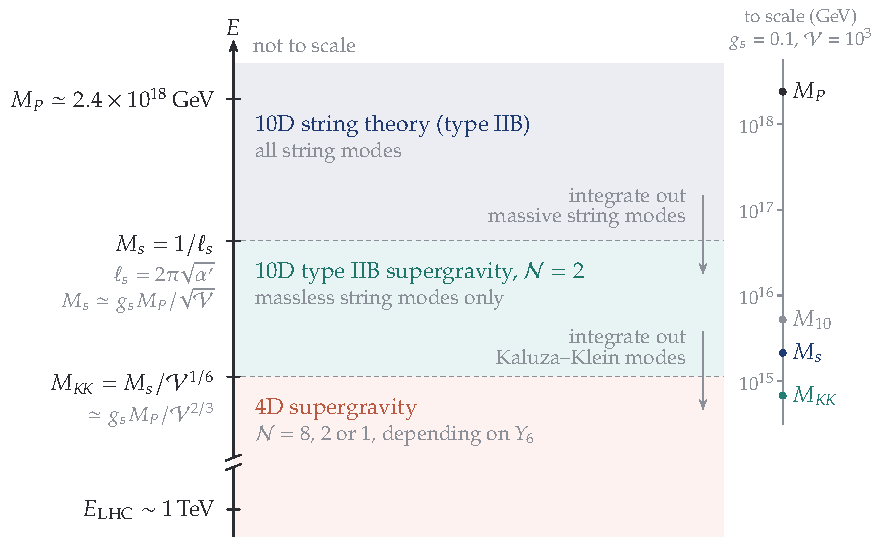
\includegraphics{fig_L1-scales}
  \caption{The hierarchy of scales of a string compactification and the effective description valid in each window of energies. The ratios are fixed by $g_s$ and $\Vol$ through \cref{eq:L1-hierarchy}.}\label{fig:L1-scales}
\end{figure}

\section{How much supersymmetry survives: holonomy}
\label{sec:L1-holonomy}

The number of supersymmetries in four dimensions depends, of course, on the number of supersymmetries in ten dimensions, but it also depends on the topology of $Y_6$. The supersymmetry generators are spinors: in type IIB supergravity two ten-dimensional Majorana--Weyl spinors. Given one such spinor in ten dimensions, one can ask how many four-dimensional spinors it corresponds to, and the answer depends on the compact space. This is what singles out the famous Calabi--Yau manifolds. The statements in this section are made in words; we shall prove them later in this part of the course.

Consider first the simplest situation, a flat internal manifold, the six-dimensional torus $T^6$. In this case the largest amount of supersymmetry is preserved: one Majorana--Weyl spinor in ten dimensions corresponds to four spinors in four dimensions, and the two of type IIB give four-dimensional $\mathcal N=8$ supergravity,
\begin{equation}
  Y_6 = T^6 ,\quad \Hol(T^6) = \{\one\}
  \qquad\Longrightarrow\qquad \text{4D } \mathcal N=8 .
  \label{eq:L1-T6}
\end{equation}
The property of $T^6$ that matters here is that it is a space of trivial \emph{holonomy}: its holonomy group contains only the identity.

The holonomy is a simple notion. Take a manifold, choose a closed path in it starting and ending at a point $p$, take a vector at $p$ and parallel-transport it around the path, as in \cref{fig:L1-holonomy}. When it gets back to $p$ the vector has the same length, but it need not be the same vector. On a flat manifold it always comes back to itself, but on a curved manifold it is in general rotated. A different closed path gives in general a different rotation. The \emph{holonomy group} is the set of all the transformations that relate the original vector to the transported one, for all possible closed paths. If the holonomy group contains only the identity, the vector always comes back to itself, as in the flat case; this is the trivial situation of the torus, which is flat.

\begin{figure}[tbp]
  \centering
  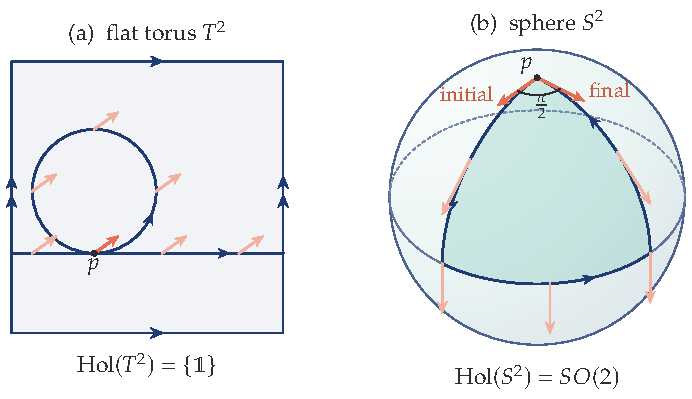
\includegraphics{fig_L1-holonomy}
  \caption{Parallel transport around closed loops. On a flat torus a vector always returns to itself, so the holonomy is trivial. On a sphere a vector carried around a closed loop returns rotated, here by $\pi/2$; the holonomy group collects all such rotations.}\label{fig:L1-holonomy}
\end{figure}

Now notice the beauty of this result. In the supersymmetry course we saw that $\mathcal N=8$ is the largest amount of supersymmetry a four-dimensional theory can have: beyond it, the supermultiplets contain massless particles of spin higher than two, which have no consistent interactions and are not seen in nature. String theory never gives more than $\mathcal N=8$, so a consistent theory reproduces this result automatically. Compactification of type IIB string theory on $\R^{1,3}\times T^6$ is a perfectly good solution of the theory. But it does not describe our world, because $\mathcal N=8$ is too much supersymmetry. The world needs at most $\mathcal N=1$ at high energies: in four-dimensional theories with $\mathcal N\ge2$ the fermions cannot be chiral, while those of the Standard Model are (see also \cref{sec:L1-questions}). The supersymmetry must be reduced, and the way to reduce it is what selects Calabi--Yau manifolds.

If instead of $T^6$ the space $Y_6$ is a \emph{Calabi--Yau manifold}, whose holonomy group is $SU(3)$, then one Majorana--Weyl spinor in ten dimensions gives a single spinor in four dimensions, and type IIB gives four-dimensional $\mathcal N=2$ supergravity:
\begin{equation}
  Y_6 = \text{Calabi--Yau} ,\quad \Hol(Y_6) = SU(3)
  \qquad\Longrightarrow\qquad \text{4D } \mathcal N=2 .
  \label{eq:L1-CY}
\end{equation}
This is why Calabi--Yau manifolds, the six-dimensional manifolds of $SU(3)$ holonomy, became famous: they break the largest possible amount of supersymmetry while preserving some of it, which is what is needed to make contact with the real world.

\begin{addition}
\emph{Why the holonomy decides.} On $\R^{1,3}\times Y_6$ the ten-dimensional Lorentz group is broken to $SO(1,3)\times SO(6)$, and the Majorana--Weyl representation $\mathbf{16}$ of $SO(1,9)$ decomposes as
\begin{equation}
  \mathbf{16} = (\mathbf 2,\mathbf 4)\oplus(\bar{\mathbf 2},\bar{\mathbf 4}) ,
  \label{eq:L1-spinor-decomp}
\end{equation}
where $\mathbf 2$ and $\bar{\mathbf 2}$ are the two Weyl spinors of $SO(1,3)$, and $\mathbf 4$ and $\bar{\mathbf 4}$ the two chiral spinors of $SO(6)$, the fundamental and antifundamental of $SU(4)\simeq\mathrm{Spin}(6)$. The Majorana condition relates the two terms, so a ten-dimensional supersymmetry parameter has the form $\epsilon(x,y) = \zeta(x)\otimes\eta(y) + \text{c.c.}$, with $\zeta$ a four-dimensional Weyl spinor and $\eta$ a spinor on $Y_6$. A supersymmetry is preserved by the background if the variations of the fermions vanish in it. With no fluxes and a constant dilaton the only condition comes from the gravitino, $\delta\psi_M = \nabla_M\epsilon = 0$, which requires $\eta$ to be covariantly constant on $Y_6$, $\nabla_m\eta = 0$. A covariantly constant spinor is unchanged by parallel transport around any loop, so it is a singlet of $\Hol(Y_6)$ acting on the $\mathbf 4$. Each such singlet $\eta$ gives one four-dimensional supersymmetry for each ten-dimensional Majorana--Weyl generator. For $T^6$ all four components are singlets, and type IIB gives $2\times4 = 8$ supersymmetries. For $\Hol = SU(3)\subset SU(4)$, $\mathbf 4\to\mathbf 3\oplus\mathbf 1$ has a single singlet, and type II gives $\mathcal N=2$; the heterotic and type I strings, which have a single Majorana--Weyl supersymmetry in ten dimensions, give $\mathcal N=1$ directly, which is how Calabi--Yau manifolds first entered string theory~\cite{CHSW} (\cref{sec:L2-heterotic}). An intermediate case is $\Hol = SU(2)$, e.g.\ $Y_6 = K3\times T^2$, with $\mathbf 4\to\mathbf 2\oplus\mathbf 1\oplus\mathbf 1$ and $\mathcal N=4$ from type II. Finally, a compact Kähler manifold of complex dimension three has $\Hol\subseteq U(3)$, and $\Hol\subseteq SU(3)$ is equivalent to Ricci-flatness; by Yau's theorem a Ricci-flat Kähler metric exists, in each Kähler class, precisely when the first Chern class vanishes. This is the usual definition of a Calabi--Yau manifold, and Ricci-flatness guarantees that the $R_6$ term dropped in \cref{eq:L1-reduction} vanishes.
\end{addition}

To reach four-dimensional $\mathcal N=1$ one more step is needed. Half of the degrees of freedom have to be projected away: one has to cut the spectrum. The operation that does it in type IIB is the \emph{orientifold projection}. It reverses the orientation of the strings and identifies different modes of the string with each other, and keeping only the combinations invariant under it projects out half of the spectrum, and with it half of the supersymmetries. Type IIB string theory on a Calabi--Yau orientifold gives four-dimensional $\mathcal N=1$ supergravity. We shall understand later in more detail what this operation means.

\begin{addition}
\emph{The orientifold projection.} Type IIB string theory is invariant under worldsheet parity $\Omega_p$, which reverses the orientation of the string and exchanges its left- and right-moving modes. Gauging this symmetry, i.e.\ keeping only the states invariant under it, gives type I string theory. In an orientifold, $\Omega_p$ is combined with an involution $\sigma$ of the compact space, $\sigma^2 = 1$, and the theory is restricted to the states invariant under the combination; the name joins ``orientation'' and ``orbifold''. For a Calabi--Yau manifold $\sigma$ is taken holomorphic and isometric, and two choices preserve four-dimensional $\mathcal N=1$~\cite{GrimmLouis}:
\begin{equation*}
  \mathcal O = (-1)^{F_L}\,\Omega_p\,\sigma^* \quad\text{with}\quad \sigma^*\Omega = -\Omega ,
  \qquad\qquad
  \mathcal O = \Omega_p\,\sigma^* \quad\text{with}\quad \sigma^*\Omega = +\Omega ,
\end{equation*}
where $\Omega$ is the holomorphic three-form of the Calabi--Yau and $(-1)^{F_L}$ the spacetime fermion number of the left-movers. The fixed loci of $\sigma$ are \emph{orientifold planes}: in the first case O3-planes, at points of $Y_6$, and O7-planes, wrapping four-cycles; in the second case O5- and O9-planes. Unlike D-branes, O-planes are not dynamical, and they carry negative tension and negative Ramond--Ramond charge. This will make them essential for the consistency (tadpole cancellation) of flux compactifications, and the O3/O7 case is the setting of the moduli-stabilisation scenarios studied later in the course.
\end{addition}

All these statements hold at the compactification scale. This scale, as we have seen, is not known, but it is expected to be very high, perhaps $10^{18}$, $10^{16}$ or $10^{15}\GeV$. At that scale, depending on the manifold on which the theory is compactified, one has four-dimensional $\mathcal N=8$, $\mathcal N=2$ for a Calabi--Yau, or $\mathcal N=1$ for a Calabi--Yau orientifold. The remaining task is then to break the last $\mathcal N=1$ to $\mathcal N=0$, at low energy, around the TeV scale, and dynamically.

The plan of this part of the course is to explain these steps: start from ten-dimensional type IIB supergravity and see how to go down to four-dimensional theories with $\mathcal N=8$, $\mathcal N=2$ and finally $\mathcal N=1$, discussing along the way the geometric notions, such as holonomy, that they require.

\section{Questions and discussion}
\label{sec:L1-questions}

The lecture ended with questions from the students. We reproduce them here with the answers, because they touch on themes that will return throughout the course.

\question{Do we have any reason to think that $g_s$ is small?}

There is no a priori reason for the string coupling to be small. The region $g_s\ll1$ is the one in which we can perform computations, but nature does not need to be in the region where we can compute. There are, however, indications that it is small, and they come from observation: everything we see in nature so far looks weakly coupled. There are many small numbers in what we know. The electromagnetic coupling $\alpha_{\mathrm{em}} = e^2/4\pi$ is about $1/137$ at the energies of our experiments; the Yukawa couplings are small, that of the electron being $y_e\simeq3\times10^{-6}$; in cosmology, the density fluctuations of the cosmic microwave background are of order $10^{-5}$. We shall see that gauge and Yukawa couplings are functions of the string coupling (and of the other moduli), so their smallness is an indication that $g_s$ is small.

But the dilaton is a field, and a field can have different configurations, different vacua. Some vacua may correspond to universes in which $g_s$ is large. They would still be solutions of string theory, just not our universe, and in fact in most of the solutions we know $g_s$ is not small. Once there are different solutions one must also understand, cosmologically, why one of them is realised in nature rather than another, or whether several are, in which case we are in a kind of multiverse and must ask how our universe is connected to the other parts. These are deep questions.

Small $g_s$ is also required from the point of view of the theory, to trust the computations, so the phenomenological and the theoretical requirements point in the same direction. In principle one would start from ten-dimensional string theory and compute all quantum effects: a tree-level part, loop corrections and non-perturbative corrections. Dimensionally reducing the full result would then give the complete four-dimensional $\mathcal N=1$ theory, with all quantum effects included. This is unfeasible. If the string coupling is small, however, one can keep only the leading-order result, knowing that the corrections one cannot compute are negligible. As said above, this is an assumption that has to be checked: the dilaton turns out to be a scalar field in four dimensions, one has to compute its potential and find where it has a minimum, since cosmologically the field is expected to end up there, and that minimum must lie at weak coupling. In most solutions this is not the case, but we shall see that in a subset of solutions it is guaranteed. We focus on those, both for the consistency of the theory and because they are good candidates to reproduce the Standard Model.

\question{If we had started from type IIA, which is not chiral in ten dimensions, could we still obtain a chiral theory in four dimensions?}

Yes: one can also start from type IIA and obtain chiral four-dimensional theories. Chirality depends on the dimension: when we say that the world is chiral we mean that it is chiral in four dimensions, and a theory that is chiral in ten dimensions need not be chiral in four. Type IIB, for instance, is chiral in ten dimensions, but compactified on $T^6$ it gives four-dimensional $\mathcal N=8$ supergravity, which is not chiral. A four-dimensional theory can be chiral only when it has $\mathcal N=1$ (or no supersymmetry). Type IIA is not chiral in ten dimensions, but when it is compactified down to four-dimensional $\mathcal N=1$ it can give a chiral theory as well. The reason why people mostly focus on type IIB rather than type IIA is that the latter is technically more complicated, not that it is excluded; we shall come back to this.

\question{The real requirement of the worldsheet theory is not ten dimensions but a central charge $c=15$. Are there options we are not considering, some conformal field theory that is not geometrical?}

Yes. The worldsheet conformal field theory describing the ``matter'' must have $c=15$, and ten free bosons with their fermionic partners are only one way of achieving it. One should think of string theory, or M-theory, as a big space of theories in which one can move, finding different configurations. At some points the configuration can be described geometrically, as $\R^{1,9}$ or as $\R^{1,3}\times Y_6$; at other points there is no geometric description. An example is the limit in which the volume of the extra dimensions goes to zero, where one finds conformal field theory limits with no geometric interpretation.

\question{Is there a reason to believe that our universe is not in one of these limits?}

Yes. In those limits there is no hierarchy. All scales are of order the string scale, and all couplings are of order one. To reproduce our universe one needs hierarchies: the string scale below the Planck scale, supersymmetry broken at a much lower scale, couplings that are small.

\begin{addition}
The counting behind $c=15$ is the one of the addition after \cref{eq:L1-D10}: the ghosts contribute $-26+11=-15$, so the rest of the worldsheet theory must contribute $+15$, with $\mathcal N=1$ worldsheet supersymmetry. In a compactification $\R^{1,3}\times Y_6$ the four flat directions contribute $\tfrac32\times4=6$, and the internal theory must have $c=9$. For a Calabi--Yau this is a supersymmetric sigma model on $Y_6$, but any conformal field theory with $c=9$ (and, for spacetime supersymmetry, $\mathcal N=2$ worldsheet supersymmetry) will do. A famous example is the Gepner model, built from $\mathcal N=2$ minimal models, which describes the quintic Calabi--Yau at a point of small volume where the geometric description has broken down.
\end{addition}

A remark of the lecturer's own belongs here. Everything said so far is put in by hand. We have assumed the background $\R^{1,3}\times Y_6$ and allowed deformations of $Y_6$: it can be a torus or a Calabi--Yau manifold, and we shall allow the Calabi--Yau to change in size, for example to have a different volume, or in shape. A change of shape at fixed size is like deforming a doughnut into a teacup: there is still one hole, one handle, and the volume may stay the same, but the shape changes. These deformations will be the moduli of the compactification (\cref{sec:L2-moduli}). It would be very nice to understand dynamically why we end up in this background rather than in something else, for example $\R^{1,4}\times Y_5$, but this is very hard, and we are not able to do it yet: it requires the whole non-perturbative M-theory, not perturbative string theory.

\question{Why do we need to understand M-theory to determine $Y_6$?}

Think of the difference between first and second quantisation in quantum field theory. The first-quantised description is the worldline formalism, in which one follows one particle at a time; to describe as many particles as one likes one needs a quantum field theory. In the first part of the course the string was introduced as a generalisation of the worldline, the worldsheet, and this formulation of string theory is a kind of first-quantised version. What one would like is a string field theory, with a field whose excitations are strings, and a complete formulation of this kind, able to describe the theory non-perturbatively, is not available.

\question{Would matrix theories, such as the BFSS model, count as string field theories?}

Matrix theories, such as the BFSS matrix model of Banks, Fischler, Shenker and Susskind, in which M-theory is described by the quantum mechanics of a large number of D0-branes, are proposals for the heart of M-theory, and branes play a crucial role in them; there are many papers on these proposals, but no consensus on the right formulation. The point is that what we can actually do is perturbative, and a simple way to see the problem is a quantum-mechanical system with two vacua. Everything we have done here studies one vacuum. Perturbation theory around it allows us to deform it, for instance to deform the Calabi--Yau, but never to reach the other vacuum, which could be, say, $\R^{1,4}\times Y_5$. What interpolates between two vacua in quantum mechanics is an instanton, a tunnelling effect, which is non-perturbative because it is not a small perturbation around either vacuum, and to describe it one needs the whole picture. Perturbative string theory around one vacuum gives, at low energy, one quantum field theory, for instance four-dimensional $\mathcal N=1$ supergravity from type IIB; around another vacuum, another quantum field theory. Connecting the two, and understanding cosmologically how the different vacua were populated in the first place, would require a description that interpolates between the different solutions of string theory.

\question{In such a description, should one see a smooth transition from, say, type IIB to the $E_8\times E_8$ heterotic string?}

Yes, one should. But the situation is even more complicated than this. Even without leaving type IIB, string theory gives many, many solutions, the landscape. They were found within type IIB because this is the limit in which computations can be done and things are under control. Sticking to this setting, one finds many different quantum field theories, all based on Calabi--Yau manifolds (more precisely, orientifolds) in type IIB, differing by the fluxes that we shall meet later; and relating them to each other, even within type IIB, would require understanding all possible connections between vacua.

The present approach is more humble. Out of all the solutions, let us at least find one that looks like our universe: one with non-abelian gauge theories like the Standard Model, the right cosmology, and so on. There are many that look like our universe. The second question is what happens to the other solutions. This question can be asked regardless of string theory, and in quantum field theory the situation is even worse: one can write down infinitely many quantum field theories, changing the gauge group or the spectrum of fields, all perfectly viable as quantum field theories, but disconnected from one another; the choice is just ours. In string theory we do not yet know how many consistent solutions there are, but at the moment their number seems to be finite, and in principle one can understand, quantum mechanically and at the non-perturbative level, how they are connected. We are far from that. A more immediate programme, in the most promising setting for phenomenology, is to study all the possible solutions and understand their common features, and then to see whether they lead to predictions: if all of them contain a new particle that we should see in nature, for example, or if none of them does, one can confront this with data.

\chapter{String phenomenology: from the heterotic string to the moduli problem}
\label{ch:L2}
\lecturedate{Lecture of 6 November 2026}

This lecture continues the general description, begun in \cref{ch:L1}, of how string theory can be connected with the real world; like the first, it is mostly qualitative. It has three parts. The first explains why we look for compactifications that preserve four-dimensional $\mathcal N=1$ supersymmetry at the Kaluza--Klein scale. The second surveys the five superstring theories in ten dimensions, the dualities that relate them and their massless spectra, and uses them to explain why string phenomenology started with the heterotic string and why it later moved to type II theories. The third introduces a problem that every string compactification has to face, and around which much of this course is organised: the \emph{moduli}, massless scalar fields that parametrise the size and the shape of the extra dimensions, and the need to stabilise them.

\section{Why four-dimensional \texorpdfstring{$\mathcal N=1$}{N=1} supersymmetry}
\label{sec:L2-N1}

In the chain of effective theories of \cref{sec:L1-hierarchy} (\cref{fig:L1-scales}), type IIB string theory gives type IIB supergravity below the string scale, and a four-dimensional supergravity below the Kaluza--Klein scale, once the Kaluza--Klein towers (\cref{sec:L1-KK}) are integrated out; how many supersymmetries survive depends on the topology of $Y_6$ (\cref{sec:L1-holonomy}). We pick Calabi--Yau manifolds, to be defined properly later, because they break the largest amount of supersymmetry while preserving some of it, and, after the orientifold projection, lead to $\mathcal N=1$ at the Kaluza--Klein scale.

One could also consider compactifications that break supersymmetry completely, with $\mathcal N=0$ at the Kaluza--Klein scale, and do model building directly there. We do not, for four reasons.

The first is that $\mathcal N=1$ is the only chiral version of four-dimensional supersymmetry: in theories with $\mathcal N\ge2$ the fermions come in non-chiral representations (\cref{sec:L1-holonomy}). With $\mathcal N=1$ there is hope of obtaining the Standard Model, which is a chiral theory.

The second concerns the scale of supersymmetry breaking. The Kaluza--Klein scale is not known: it could be close to the TeV scale, at the edge of detection, but more realistically it is very high, say $10^{14}$--$10^{15}\GeV$. The $\mathcal N=1$ supersymmetry that survives there should then be broken spontaneously at much lower energies, for example at the TeV scale, to address the hierarchy problem, and \emph{dynamically}: the hope is that non-perturbative effects, as in confinement, generate a scale exponentially smaller than the fundamental ones. Supersymmetry broken at low energies has the good properties met in the supersymmetry course: it addresses the hierarchy problem, provides a dark matter candidate, leads to radiative electroweak symmetry breaking, in which loop corrections break the electroweak symmetry dynamically, and makes the gauge couplings unify. The hope is to recover all of these from a top-down approach. Whether this works is a property of the effective theory: one has to derive it from string theory, compute the non-perturbative effects, and check whether they break the remaining $\mathcal N=1$ at low energies. It might also turn out that this is never possible.

The third concerns how the breaking is communicated. Besides knowing whether supersymmetry is broken at low energies, one must understand how the breaking is mediated to the \emph{visible sector}, the supersymmetric version of the Standard Model, for instance the minimal supersymmetric Standard Model (MSSM). Some other sector of the compactification is responsible for breaking supersymmetry, and it must couple to the MSSM in such a way that the MSSM feels the breaking and the supersymmetric partners become massive. The breaking felt by the MSSM must be \emph{soft}, so that the cancellation of quadratic divergences survives, and soft supersymmetry breaking is generated naturally in supergravity theories derived from string theory, through gravitational interactions. This is \emph{gravity mediation}.

These three reasons are phenomenological. The fourth is theoretical, and we have not met it yet in the supersymmetry course: \emph{$\mathcal N=1$ supersymmetry allows one to control the quantum corrections to the effective theory.} A supersymmetric theory is specified by its Kähler potential $K$ and its superpotential $W$, and one can ask how these quantities behave under quantum corrections. Each of them has a tree-level part, loop corrections and non-perturbative corrections, but not on the same footing:
\begin{equation}
  K = K_{\text{tree}} + K_{\text{loops}} + K_{\text{np}} ,\qquad
  W = W_{\text{tree}} + W_{\text{np}} .
  \label{eq:L2-KW}
\end{equation}
The superpotential is exact at tree level in perturbation theory: as a consequence of supersymmetry and of holomorphy it receives no loop corrections, only non-perturbative ones (this will be proved in the supersymmetry course). This is a very powerful result: once $W$ is computed at tree level, one knows for sure that there are no loop corrections. The Kähler potential, instead, does receive loop corrections. Since computing quantum corrections in string theory is extremely hard, this control is very important, and in a compactification that breaks supersymmetry completely it is absent. Keeping some supersymmetry helps to compute the effective theory, but not too much of it: with $\mathcal N=1$, and not $\mathcal N=2$, the theory remains chiral and good for phenomenology. That is the balance.

In an $\mathcal N=0$ compactification a ten-dimensional Majorana--Weyl spinor corresponds to no spinor at all in four dimensions, so a ten-dimensional supersymmetry generator gives nothing. An example is $Y_6 = S^6$, a six-dimensional sphere, whose holonomy group is $SU(4)$ in the lecture's words, to be compared with $SU(3)$ for a Calabi--Yau manifold.
Why the holonomy group determines the number of four-dimensional supersymmetries will be explained towards the end of the course.

\section{Five superstring theories and their dualities}
\label{sec:L2-dualities}

Our starting point will be ten-dimensional type IIB string theory, because, as we shall try to explain, it is at present the most promising one for phenomenology. In the end the starting point does not matter much, since all string theories are related by dualities. What changes from one description to another is which quantities are easy to compute: something that looks weakly coupled, and so computable, in one description can look strongly coupled, and hard to compute, in another.

The five consistent perturbative superstring theories recalled in \cref{sec:L1-aims}, type IIA, type IIB, type I and the two heterotic theories, with gauge groups $SO(32)$ and $E_8\times E_8$, are all related by dualities of two kinds. \emph{S-dualities} are strong--weak coupling dualities: they act on the dilaton, and exchange a theory at string coupling $g_s$ with one at coupling $1/g_s$. \emph{T-dualities} act instead on the geometry: they change the radius of the compactification manifold. The five theories are therefore best thought of not as different theories but as different limits, or better different perturbative corners, of a single, more fundamental theory, \emph{M-theory}. What we know of M-theory is its low-energy limit, eleven-dimensional supergravity. In it, the size of the eleventh dimension corresponds to the string coupling. In a perturbative corner, where the coupling goes to zero and perturbation theory can be used, the size of the eleventh dimension goes to zero, and one recovers a ten-dimensional theory; when the coupling becomes large, one starts to see the eleventh dimension.

The simplest example is the relation between M-theory and type IIA. Compactified on a circle $S^1$ of radius $R$, going from eleven to ten dimensions, M-theory gives type IIA string theory, and $R$ is set by the dilaton in such a way that
\begin{equation}
  R\to0 \qquad\Longleftrightarrow\qquad g_s\to0 \qquad\text{(type IIA limit)} .
  \label{eq:L2-IIA-limit}
\end{equation}
Type IIA is in turn T-dual to type IIB. T-duality changes the size of the compactification manifold: type IIA compactified on a circle of radius $R$ is the same theory as type IIB compactified on a circle of radius
\begin{equation}
  \tilde R = \frac{\alpha'}{R} = \frac{1}{4\pi^2\Ms^2R} .
  \label{eq:L2-Tduality}
\end{equation}
The two are the same theory, with $R$ exchanged for $\alpha'/R$: an example of a duality. The whole web of dualities is shown in \cref{fig:L2-dualities}.

\begin{figure}[tbp]
  \centering
  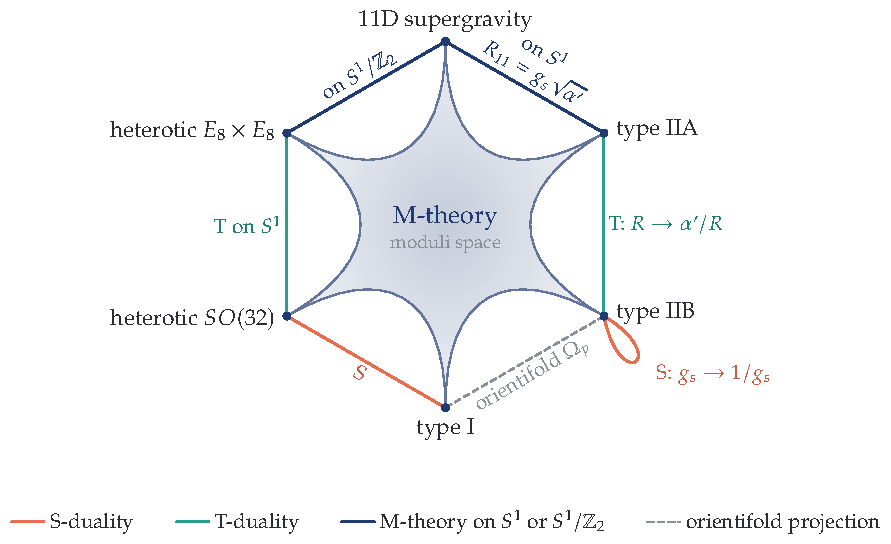
\includegraphics{fig_L2-dualities}
  \caption{The five ten-dimensional superstring theories and eleven-dimensional supergravity as limits of a single theory, M-theory, and the dualities that relate them.}\label{fig:L2-dualities}
\end{figure}

\section{Massless spectra and the first string models}
\label{sec:L2-spectra}

String phenomenology, the attempt to obtain the real world from string theory, started in the mid-1980s: string theory was born at the end of the 1960s and developed in the 1970s, and in the mid-1980s people started trying to connect it with the real world.

These first attempts used not type IIB but the $E_8\times E_8$ heterotic string. The type II theories seemed to give no non-abelian gauge bosons in four dimensions, which are needed for the Standard Model, and so, although consistent, they seemed unfit for the real world. The heterotic string, instead, has a gauge group in its massless spectrum, $E_8\times E_8$, and $E_8$ is a huge group which contains the Standard Model gauge group. The idea was to break one $E_8$ factor down to the Standard Model with a Higgs mechanism, and to use the dynamics of the other to break supersymmetry. This programme turned out to be very hard, for reasons explained below, although heterotic phenomenology is still pursued today. Around 1995 came the discovery of \emph{D-branes} as dynamical objects of string theory, and with it the realisation that the open strings ending on them can behave as non-abelian gauge bosons (\cref{sec:L4-gauge}). D-branes are present in type II theories, so one had simply missed an ingredient: the non-abelian gauge bosons are absent from the closed-string spectrum, but they can come from open strings. Since then type II theories have been studied more than the heterotic string for phenomenology.

To see why, we list the massless modes of the closed string and the ten-dimensional fields they correspond to, in \cref{tab:L2-spectra}, for type IIA, type IIB and the heterotic string.

\begin{table}[tbp]
  \centering
  \renewcommand{\arraystretch}{1.35}
  \begin{tabular}{@{}llll@{}}
    \toprule
    Sector & Type IIA & Type IIB & Heterotic \\
    \midrule
    NS--NS & $G_{MN},\ B_{MN},\ \phi$ & $G_{MN},\ B_{MN},\ \phi$ & $G_{MN},\ B_{MN},\ \phi,\ A^a_M$ \\
    R--R   & $C_1,\ C_3$ & $C_0,\ C_2,\ C_4$ & --- \\
    NS--R  & $\psi^1_{M+},\ \lambda^1_-$ & $\psi^1_{M+},\ \lambda^1_-$ & $\psi_{M+},\ \lambda_-,\ \lambda^a_+$ \\
    R--NS  & $\psi^2_{M-},\ \lambda^2_+$ & $\psi^2_{M+},\ \lambda^2_-$ & --- \\
    \midrule
    10D supersymmetry & $\mathcal N=2$, non-chiral & $\mathcal N=2$, chiral & $\mathcal N=1$, chiral \\
    \bottomrule
  \end{tabular}
  \caption{Massless spectra of the type IIA, type IIB and heterotic superstrings in ten dimensions, sorted by sector: the first label refers to the left-movers, the second to the right-movers (for the heterotic string see the text). $G_{MN}$ is the metric, $B_{MN}$ the Kalb--Ramond two-form, $\phi$ the dilaton, $C_p$ the R--R $p$-forms, $\psi_M$ the gravitini, $\lambda$ the dilatini; $A^a_M$ and $\lambda^a$ are the heterotic gauge bosons and gaugini, $a = 1,\dots,\dim G = 496$, with $G = SO(32)$ or $E_8\times E_8$. The subscripts $\pm$ give the ten-dimensional chirality.}
  \label{tab:L2-spectra}
\end{table}

The labels NS and R stand for Neveu--Schwarz and Ramond, and they are boundary conditions for the fermions on the worldsheet. The bosonic coordinates $X^M(\sigma)$ of a closed string must come back to themselves when one goes around the string, $\sigma\to\sigma+2\pi$. When the theory is supersymmetrised one must add worldsheet fermions $\psi^M$, and these can come back either to themselves or to minus themselves:
\begin{equation}
  \psi^M(\sigma+2\pi) = +\psi^M(\sigma)\quad\text{(Ramond)} ,\qquad
  \psi^M(\sigma+2\pi) = -\psi^M(\sigma)\quad\text{(Neveu--Schwarz)} .
  \label{eq:L2-NSR}
\end{equation}
On a closed string there are left-movers and right-movers, and the condition can be chosen independently for each. In type II theories there are worldsheet fermions for both, and so two spacetime supersymmetries, one coming from the left-movers and one from the right-movers; this is why they are called type II, and why all four combinations NS--NS, R--R, NS--R and R--NS appear. In the heterotic string there are worldsheet fermions only for the right-movers, and so only one spacetime supersymmetry. The left-movers have no worldsheet fermions at all: they are those of the bosonic string. Being bosonic, they produce only spacetime bosons, as an NS sector does, which is why the two heterotic sectors are labelled NS--NS and NS--R, according to the boundary condition of the right-movers.

Now the fields. The NS--NS sector always contains the metric $G_{MN}$, the antisymmetric Kalb--Ramond two-form $B_{MN}$ and the dilaton $\phi$, the spectrum of any bosonic string theory. The heterotic string has in addition gauge bosons $A^a_M$, ten-dimensional vectors (hence the index $M$, not $\mu$), and many of them: $a = 1,\dots,\dim G$, with $G = SO(32)$ or $G = E_8\times E_8$, both of dimension $496$ ($\dim E_8 = 248$). ($E_6$, $E_7$ and $E_8$ are the exceptional Lie groups, related to the octonions.) This is why people expected the heterotic string to work: with non-abelian gauge bosons in ten dimensions, the four-dimensional theory would inherit some of them.

In the R--R sector type IIA has a one-form $C_1$ and a three-form $C_3$, and type IIB a zero-form $C_0$, a two-form $C_2$ and a four-form $C_4$. These are differential forms, i.e.\ antisymmetric tensors, such as $C_2\leftrightarrow C_{MN} = C_{[MN]}$ and $C_4\leftrightarrow C_{MNPQ} = C_{[MNPQ]}$, and $C_0$ is a pseudoscalar. They are all bosons. There are also higher forms, but they are dual to the ones listed: a $p$-form $C_p$ in ten dimensions is equivalent to an $(8-p)$-form, since the field strengths are related by $F_{p+1} = \star F_{9-p}$, and in type IIB the field strength of $C_4$ is self-dual, $F_5 = \star F_5$.

The NS--R and R--NS sectors give fermions. There are two \emph{gravitini} $\psi_M$, of spin $3/2$, since there are as many gravitini as supersymmetries and type II theories have ten-dimensional $\mathcal N=2$, and two \emph{dilatini} $\lambda$, of spin $1/2$, the supersymmetric partners of the dilaton. The subscripts $\pm$ give the ten-dimensional chirality, the eigenvalue of $\Gamma_{11}$, the ten-dimensional analogue of $\gamma_5$. In type IIA the two gravitini have opposite chiralities, and so do the two dilatini: type IIA is a non-chiral theory in ten dimensions. In type IIB the two gravitini have the same chirality, and so do the two dilatini: type IIB is a chiral theory in ten dimensions (see also the conventions). The heterotic string has a single supersymmetry in ten dimensions, hence one gravitino and one dilatino, and in addition the supersymmetric partners of the gauge bosons, the \emph{gaugini} $\lambda^a$: it is ten-dimensional $\mathcal N=1$ supergravity coupled to super-Yang--Mills theory with gauge group $G$.

\section{Gauge bosons in four dimensions}
\label{sec:L2-vectors}

The ten-dimensional gauge bosons of the heterotic string lead, in four dimensions, to four-dimensional gauge bosons: choosing the index $M=\mu$ and keeping the zero mode, constant along $Y_6$, one obtains $A^a_\mu(x)$, non-abelian gauge bosons that can give the gluons and the $W$ and $Z$ bosons of the Standard Model. In type IIA and type IIB this is not possible, and the reason is worth understanding, because it will come back in the discussion of moduli.

A ten-dimensional two-form, an object with two indices, could give objects with one index in four dimensions. Taking for instance $M=\mu$ along $\R^{1,3}$ and $N=n$ along $Y_6$, the component $B_{\mu n}$ is, from the four-dimensional point of view, a vector labelled by $n$. To extract its massless modes one expands it in the zero modes of the internal Laplacian, which for an object with one internal index are the harmonic one-forms $\omega^I_n(y)$ of $Y_6$:
\begin{equation}
  B_{\mu n}(x,y) = \sum_I A^I_\mu(x)\,\omega^I_n(y) + \text{(massive Kaluza--Klein modes)} .
  \label{eq:L2-Bmu}
\end{equation}
One is effectively reducing $B$ on one-cycles, one-dimensional submanifolds of the Calabi--Yau. But a Calabi--Yau manifold has no harmonic one-forms, $b_1(Y_6) = 0$, so these components vanish, and neither $G_{MN}$ nor $B_{MN}$ can give a vector $A_\mu(x)$ in four dimensions. We shall see later why this is a property of the Calabi--Yau.

The R--R forms offer more possibilities. $C_1$ in type IIA is already a one-form, and gives a vector directly. A form with more indices gives a vector if it is reduced on a cycle with one dimension less than its degree: $C_3$ in type IIA reduced on a two-cycle ($3-2 = 1$), or $C_4$ in type IIB reduced on a three-cycle ($4-3=1$). In principle all of these behave in four dimensions as objects with one index.
This does not work either, for a reason that is a property of the effective theory: the R--R forms do not couple to any massless mode of the string. The photon of the Standard Model must couple to leptons and quarks, while the R--R photons couple only to objects with masses at or above the string scale, the D-branes that we shall meet in \cref{ch:L4}; moreover they are abelian. The closed-string spectrum of type II theories does give photons, but not the photon of the Standard Model.

This is an interesting prediction of string theory: on top of the ordinary photon there are many other massless abelian gauge bosons, \emph{dark photons}, dark because they do not couple to ordinary matter except gravitationally. One way to detect them uses cosmology. If they were produced in the early universe, they behave in practice like extra neutrinos: they have spin one rather than one half, but they carry no charge, are relativistic, since they are massless, and are effectively decoupled from the Standard Model. As a dark relativistic species they add to the energy density of the universe and modify its expansion rate, so measuring the expansion rate either reveals something beyond the three neutrinos or strongly constrains these models.

\section{Heterotic model building}
\label{sec:L2-heterotic}

For these reasons, in the mid-1980s people focused on the $E_8\times E_8$ heterotic string. One $E_8$ factor is the \emph{visible sector}: a symmetry breaking (a Higgs mechanism) inside it brings it down to a grand unified theory (GUT). The relevant subgroups are
\begin{equation}
  E_8 \supset SO(10) \supset SU(5) \supset SU(3)\times SU(2)\times U(1) .
  \label{eq:L2-E8-chain}
\end{equation}
$SO(10)$ and $SU(5)$ are the groups used for grand unification, and a Higgs mechanism, similar to the one that breaks $SU(2)_L\times U(1)_Y$ in the Standard Model, breaks $SU(5)$ down to $SU(3)\times SU(2)\times U(1)$. At the beginning there is a single group factor, so a single coupling: a unified theory with only one non-gravitational interaction, which then breaks down to the three interactions of the Standard Model.

The second $E_8$ factor is a \emph{hidden sector}: the leptons and quarks of the Standard Model are not charged under it, and the matter charged under it is not charged under the Standard Model. The hidden sector is responsible for supersymmetry breaking, through a dynamics very similar to confinement in QCD. In QCD the gauge coupling grows towards low energies and blows up, and quarks and antiquarks condense: the quark bilinear develops a non-zero vacuum expectation value, $\langle q\bar q\rangle\neq0$. Similarly, strong dynamics at low energies in the hidden $E_8$ gives a non-zero vacuum expectation value to some fields and breaks supersymmetry. Gravitational interactions, which are always present, then mediate the breaking to the visible sector, which becomes a non-supersymmetric Standard Model. That was the idea.

\section{The problems of the heterotic string: the GUT coupling}
\label{sec:L2-alphaGUT}

The heterotic string, however, has problems that have not yet been fully addressed. The first concerns the gauge coupling. In a heterotic compactification that leads to a grand unified theory, based on $SO(10)$ or $SU(5)$, the GUT coupling is controlled by the string coupling and by the volume of the Calabi--Yau manifold in string units (for now, take it for granted):
\begin{equation}
  \alpha_{\mathrm{GUT}} \equiv \frac{g_{\mathrm{GUT}}^2}{4\pi} \simeq \frac{g_s^2}{\Vol} .
  \label{eq:L2-alphaGUT}
\end{equation}
From phenomenology, on the other hand, we know the value of $\alpha_{\mathrm{GUT}}$: the three gauge couplings of the Standard Model, run with the renormalisation group of the MSSM, tend to unify at
\begin{equation}
  \alpha_{\mathrm{GUT}}^{-1}\simeq25 ,
  \label{eq:L2-alphaGUT-value}
\end{equation}
as shown in \cref{fig:L2-unification}.

\begin{figure}[tbp]
  \centering
  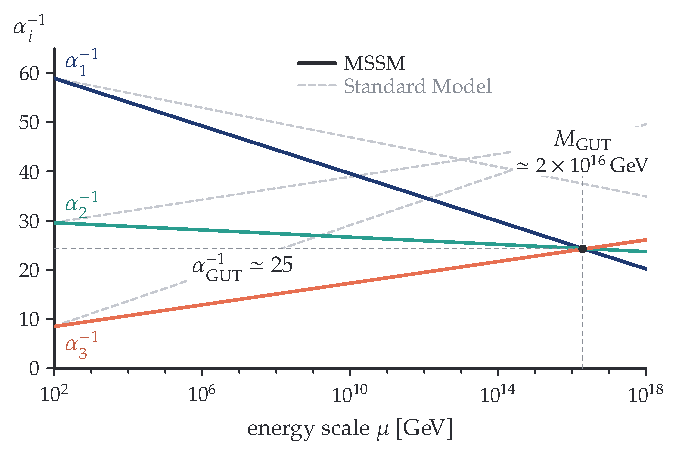
\includegraphics{fig_L2-unification}
  \caption{Running of the three inverse gauge couplings of the Standard Model gauge group with the MSSM spectrum, at one loop. They meet at $\alpha^{-1}_{\mathrm{GUT}}\simeq 25$ at $M_{\mathrm{GUT}}\simeq2\times10^{16}\GeV$.}\label{fig:L2-unification}
\end{figure}

But then \cref{eq:L2-alphaGUT} requires
\begin{equation}
  \Vol \simeq 25\,g_s^2 ,
  \label{eq:L2-V25}
\end{equation}
so one cannot have at the same time $g_s\ll1$ and $\Vol\gg1$, the two conditions of \cref{eq:L1-hierarchy-conditions} for trusting the effective theory. At small string coupling the volume is of order one or smaller, and the higher-derivative ($\alpha'$) corrections are very large; at large volume, where they are suppressed, the string coupling is large, and the loop corrections can never be ignored. Either way it is hard to trust the effective theory. We shall see that type II theories avoid this problem. There the gauge fields live on D-branes, and their coupling is set by the size of the cycle that the branes wrap, not by $\Vol$, so one can go to large volume and small string coupling while keeping $\alpha_{\mathrm{GUT}}^{-1}\simeq25$.

\section{Moduli}
\label{sec:L2-moduli}

The second problem introduces a concept that applies to every string theory, not only to the heterotic string: \emph{moduli stabilisation}. Consider the dimensional reduction of the ten-dimensional metric to four dimensions. Starting from one metric in ten dimensions, one obtains many scalars in four dimensions, the \emph{moduli}. On $X_{10} = \R^{1,3}\times Y_6$ (\cref{eq:L1-X10}), with coordinates $x^\mu$ on $\R^{1,3}$ and $y^m$ on the Calabi--Yau manifold $Y_6$, the metric $G_{MN}(x,y)$ splits into three kinds of components:
\begin{equation}
  G_{MN}(x,y) \longrightarrow
  \begin{cases}
    G_{\mu\nu}(x) , \\[0.5ex]
    G_{\mu m}(x,y) = \sum_I A^I_\mu(x)\,\omega^I_m(y) = 0 \quad\text{for a Calabi--Yau} , \\[0.5ex]
    G_{mn}(x,y) = \sum_I \phi^I(x)\,\omega^I_{mn}(y) .
  \end{cases}
  \label{eq:L2-metric-split}
\end{equation}
The first, with both indices along $\R^{1,3}$, gives the four-dimensional metric. The mixed components $G_{\mu m}$ are four-dimensional vectors, whose zero modes would come from the harmonic one-forms $\omega^I_m(y)$ of $Y_6$, exactly as for $B_{\mu n}$ in \cref{eq:L2-Bmu}. A Calabi--Yau has none ($b_1=0$, \cref{sec:L2-vectors}), so the metric gives no vectors.

The internal components $G_{mn}$ are four-dimensional scalars, since $m$ and $n$ are just labels. They are expanded in scalar fields $\phi^I(x)$ times objects $\omega^I_{mn}(y)$ with two internal indices, and the number of terms is a topological property of $Y_6$: in practice $I$ takes hundreds of values. A metric in ten dimensions therefore gives a metric in four dimensions plus many scalars, which parametrise the internal metric: moving in the space of these fields changes the size or the shape of the Calabi--Yau, as anticipated at the end of \cref{sec:L1-holonomy}. Mathematicians call such parameters of the Calabi--Yau metric moduli; in physics they are scalar fields. One of them is the volume $\Vol$ that appears in $\alpha_{\mathrm{GUT}}$, \cref{eq:L2-alphaGUT}. As a field, $\Vol(x)$ is a function on Minkowski space: the Calabi--Yau attached at the point $x$ can have a different volume from the one attached at another point.

There are, in general, three types of moduli.

\emph{Kähler moduli.} The first type parametrises deformations of the size of $Y_6$; an example is the volume. They are denoted
\begin{equation}
  T_i(x) ,\qquad i = 1,\dots,h^{1,1}(Y_6) ,
  \label{eq:L2-T}
\end{equation}
where $h^{1,1}$, a \emph{Hodge number}, is the number of linearly independent harmonic $(1,1)$-forms on $Y_6$, those annihilated by the Laplacian, $\Delta\omega = 0$: a topological property. The name $(1,1)$ comes from the fact that $Y_6$ is a complex manifold, on which one can use holomorphic and antiholomorphic coordinates $z^i$ and $\bar z^{\bar\imath}$, as one describes the plane either with $(x,y)$ or, as the complex plane, with $(z,\bar z)$. A $(1,1)$-form has one holomorphic and one antiholomorphic index, $\omega_{i\bar\jmath}\,\dd z^i\wedge\dd\bar z^{\bar\jmath}$.

\emph{Complex-structure moduli.} The second type changes the complex structure of $Y_6$, i.e.\ how complex coordinates are assigned to it. Without changing the volume, these deformations change the shape of $Y_6$. They are denoted
\begin{equation}
  U_a(x) ,\qquad a = 1,\dots,h^{2,1}(Y_6) ,
  \label{eq:L2-U}
\end{equation}
where the Hodge number $h^{2,1}$ counts the linearly independent harmonic $(2,1)$-forms on $Y_6$. The beauty of the construction is that topological properties of $Y_6$ correspond to new scalar fields in four dimensions.

\emph{The axio-dilaton.} The third type comes not from the metric but from the other scalars of the massless spectrum of type IIB, \cref{tab:L2-spectra}: the dilaton $\phi$ and the R--R zero-form $C_0$, a scalar since it has no index. They combine into a complex scalar, the \emph{axio-dilaton}
\begin{equation}
  S = e^{-\phi} + i\,C_0 .
  \label{eq:L2-S}
\end{equation}
All the moduli turn out to be complex: $T_i$ and $U_a$, like $S$, are complex scalar fields. The real part of $S$ is $e^{-\phi}$, so by \cref{eq:L1-gs} its expectation value is the inverse string coupling,
\begin{equation}
  \langle\mathrm{Re}\,S\rangle = \frac{1}{g_s} \gg 1 ,
  \label{eq:L2-ReS}
\end{equation}
which must be large for the effective theory to be trusted.

For a typical Calabi--Yau manifold both $h^{1,1}$ and $h^{2,1}$ can be of order $100$, so that one metric in ten dimensions gives hundreds of scalars in four. Calabi--Yau manifolds are named after Eugenio Calabi, an Italian-born mathematician, who conjectured their existence, and Shing-Tung Yau, a Chinese-born mathematician, who proved it; mathematicians and theoretical physicists then started building explicit examples.
Their number is still not known. The largest dataset built so far, that of Kreuzer and Skarke~\cite{KreuzerSkarke}, has about half a billion examples, $473\,800\,776$ (it lists the four-dimensional reflexive polytopes, each of which defines Calabi--Yau threefolds as hypersurfaces in a toric variety), each a good string compactification. A few have both Hodge numbers small, for instance $h^{1,1} = 1$ and a small $h^{2,1}$, and so only a few scalars, but most have many; for the compactification they are all equally good.

\section{The moduli problem}
\label{sec:L2-moduli-problem}

What happens to the physics if there are all these scalars in four dimensions? The answer is that the moduli mediate new interactions. Since in ten dimensions they are the metric, the moduli couple gravitationally to everything. This also explains why we have not seen them: they carry no charge under the Standard Model gauge group, and feel neither QCD nor the electroweak interactions. But the gravitational interaction between two massive particles is the exchange of a graviton, and on top of it there can be the exchange of any of these scalars: a fermion can emit a modulus through a gravitational vertex, and another fermion can absorb it. This is a new interaction of gravitational strength, which modifies Newton's law.

How far can this be tolerated? Newton's inverse-square law $1/r^2$ has been verified experimentally down to distances of a few tens of micrometres, which is not small at all: below that we do not know how gravity behaves, whereas the LHC probes the other interactions down to $10^{-18}\,$m. The reason is that when two bodies are pushed closer to each other the other interactions become more important, and they are hard to shield.
What this means depends on the masses of the moduli. Massless moduli modify gravity at arbitrarily large distances. Massive ones mediate a force of finite range, just as the weak interactions are felt only inside nuclei because the $W$ and $Z$ bosons are massive, and modify gravity only at short distances. To avoid these \emph{fifth forces} a string compactification must give all the moduli a mass large enough for the forces to have escaped detection. At tree level, however, all of them are massless, with nothing to give them a mass, so one has to include quantum corrections and see whether they generate a potential that does. This is the problem of \emph{moduli stabilisation}. A massless field has a flat potential, so its value is not fixed anywhere and can have very large quantum fluctuations; a potential with a minimum stabilises the field there, besides giving it a mass.

In summary, \emph{moduli are uncharged four-dimensional scalars with gravitational-strength interactions with ordinary matter, since they come from the metric, and are massless at leading (tree-level) order in supergravity.} Their potential is flat: deformations of the size and shape of the extra dimensions cost no energy. This would be a phenomenological disaster, for two reasons.

\subsection{Fifth forces}

The first reason is the one just described: massless moduli would mediate fifth forces of Yukawa type, which are not observed. The four-dimensional Lagrangian contains, together with the mass term of a fermion $\psi$ of ordinary matter, such as the electron, an interaction of Yukawa type with a modulus,
\begin{equation}
  \mathcal L_4 \supset \frac{m_\psi}{\Mp}\,\phi\,\bar\psi\psi ,
  \label{eq:L2-yukawa}
\end{equation}
where $\phi$ stands for any of the moduli, canonically normalised, and the coupling up to a coefficient of order one is shown. The suppression by the Planck mass is typical of gravitational interactions. Through this coupling the exchange of $\phi$ between two particles of ordinary matter, \cref{fig:L2-fifthforce}, gives a fifth force, with a vertex $m_\psi/\Mp$ at each end. The observational limit for moduli that couple to ordinary matter with strength $1/\Mp$ is that, to avoid these fifth forces, they must be heavier than about a meV:
\begin{equation}
  m_\phi \gtrsim 1\,\mathrm{meV} .
  \label{eq:L2-bound}
\end{equation}

\begin{figure}[tbp]
  \centering
  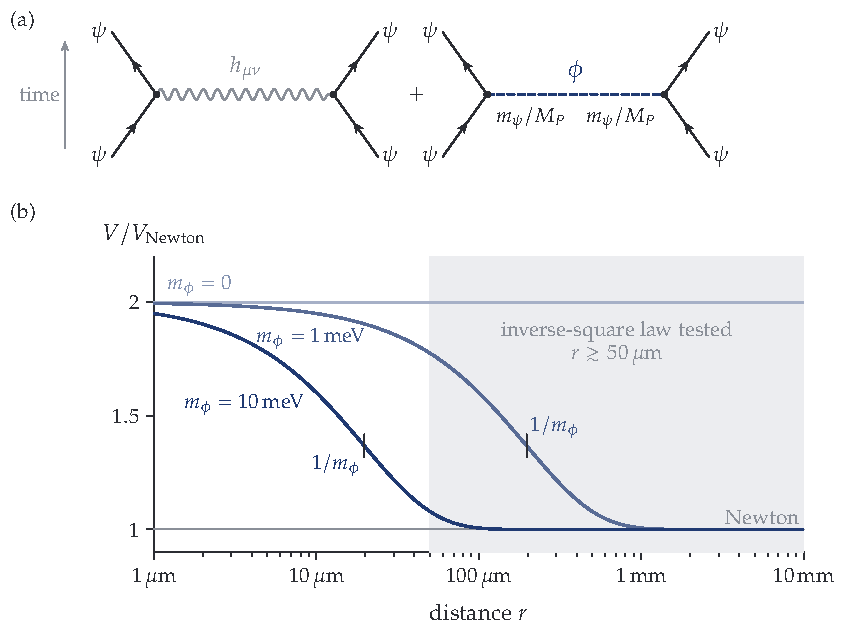
\includegraphics{fig_L2-fifthforce}
  \caption{A modulus as the mediator of a fifth force. (a) Tree-level exchange of a modulus $\phi$ between two fermions, with the coupling of \cref{eq:L2-yukawa} at each vertex, on top of the exchange of a graviton. (b) The resulting potential between two masses relative to Newton's, $V/V_{\mathrm{Newton}} = 1+\alpha_\phi\,e^{-m_\phi r}$, where $\alpha_\phi$ is the strength of the fifth force relative to gravity (here $\alpha_\phi=1$), for a massless modulus and for two massive ones.}\label{fig:L2-fifthforce}
\end{figure}

\subsection{Lack of predictivity}

The second reason is that all the features of the effective theory depend on the moduli. The only parameter that can be fixed by hand is $\alpha'$, and once it is fixed (or traded for $\Mp$, \cref{eq:L1-MP-Ms}) everything else is the vacuum expectation value of a field. For example, the coupling $\alpha_{\mathrm{GUT}}$ of \cref{eq:L2-alphaGUT}, written in terms of the moduli with \cref{eq:L2-ReS}, is
\begin{equation}
  \alpha_{\mathrm{GUT}} \simeq \frac{g_s^2}{\Vol} = \frac{1}{\langle\Vol\rangle\,\langle\mathrm{Re}\,S\rangle^2} ,
  \label{eq:L2-alphaGUT-moduli}
\end{equation}
where $\langle\Vol\rangle$ is the expectation value of the volume modulus: the coupling is the expectation value of a combination of two moduli. If these are massless, their potential is flat, any value is allowed, with huge quantum fluctuations, and $\alpha_{\mathrm{GUT}}$ cannot be predicted. The same holds for the scales of \cref{ch:L1}: the string scale $\Ms\simeq g_s\Mp/\sqrt\Vol$ (\cref{eq:L1-MP-Ms}) and the Kaluza--Klein scale $\MKK\simeq g_s\Mp/\Vol^{2/3}$ (\cref{eq:L1-MKK}) are other combinations of $g_s$ and $\Vol$. Without knowing the moduli one knows neither $\Ms$, nor $\MKK$, nor $\alpha_{\mathrm{GUT}}$: one knows nothing.

There is therefore a huge lack of predictivity, because all the features of the four-dimensional effective theory are functions of the moduli: the gauge couplings, the Yukawa couplings, the mass spectrum, the string and Kaluza--Klein scales, the scale of supersymmetry breaking, the cosmological constant, the scale of inflation, and even the gauge group. In a sense this is the beauty of string theory, since all these quantities can be predicted rather than chosen by hand; but with massless moduli nothing is predicted.

What is needed is \emph{moduli stabilisation}: the study of the quantum corrections to the scalar potential $V$ (not to be confused with the volume $\Vol$), which can develop a minimum, stabilise the moduli $\phi^I$ there, make them massive and fix the predictions,
\begin{equation}
  \frac{\partial V}{\partial\phi^I}\bigg|_{\langle\phi\rangle} = 0 ,\qquad
  m^2_{IJ}\propto\frac{\partial^2V}{\partial\phi^I\partial\phi^J}\bigg|_{\langle\phi\rangle}\ \text{positive definite} ,
  \label{eq:L2-stabilisation}
\end{equation}
with the mass matrix normalised by the kinetic terms of the moduli, and with masses large enough to satisfy \cref{eq:L2-bound} and the much stronger cosmological bound \cref{eq:L3-CMP-bound} of \cref{sec:L3-CMP}. Why this is hard in the heterotic string is the subject of \cref{sec:L3-heterotic}; a hint is already in \cref{sec:L2-alphaGUT}: there the quantum corrections are hard to control, and yet they are exactly what is needed to stabilise the moduli.

\chapter{Moduli stabilisation: the Dine--Seiberg problem and the cosmological moduli problem}
\label{ch:L3}
\lecturedate{Lecture of 12 November 2026}

This lecture completes the general picture drawn in the previous two. Many statements are still made without derivation, deliberately: the aim is an overall view of how string compactifications connect with the real world, and of what can go wrong, before the material is written down in equations, starting in the next lecture with D-branes. The lecture has three parts. The first explains why moduli stabilisation, introduced at the end of \cref{ch:L2}, is particularly hard in the heterotic string, and why type IIB is better placed. The second discusses, in a toy model with a single modulus, the general difficulty of stabilising the moduli with quantum corrections while keeping the effective theory under control, the \emph{Dine--Seiberg problem}, and the idea that resolves it. The third explains, with a simple cosmological estimate, why the moduli must be heavier than about $30\TeV$: the \emph{cosmological moduli problem}.

\section{Why moduli stabilisation is hard in the heterotic string}
\label{sec:L3-heterotic}

The moduli of \cref{sec:L2-moduli}, the Kähler moduli $T_i$, the complex-structure moduli $U_a$ and the axio-dilaton $S$, have a flat potential at tree level, which leads to fifth forces and to a complete lack of predictivity (\cref{sec:L2-moduli-problem}). Moduli stabilisation is the study of the quantum corrections that generate a potential for them, lift the flat directions and make them massive; the minimum of the potential then fixes, or \emph{stabilises}, the moduli at a point where predictions become possible.

In the heterotic string this programme is problematic, for three reasons. The first was met in \cref{sec:L2-alphaGUT}: by \cref{eq:L2-V25} the string coupling cannot be small, to suppress higher string loops, while the volume is large, to suppress higher-derivative corrections, so the effective theory is hard to trust. In type II theories one can have both; this was known from the beginning, but since type II theories seemed to give no non-abelian gauge bosons in four dimensions (\cref{sec:L2-spectra}), the advantage did not seem to matter.

\subsection{Background fluxes}

The second reason is that a major source of the potential for the moduli are \emph{background fluxes}, generalisations of electromagnetic fluxes. By Gauss's law, the flux of the electric field through a sphere surrounding a charge measures the charge, and similarly for the magnetic flux of a monopole; such fluxes carry energy. In four-dimensional Minkowski space a background electromagnetic field would pick a direction and break Lorentz invariance, but in the extra dimensions nothing forbids it: turning on fluxes there is like giving the field a vacuum expectation value in the extra dimensions, leaving the four-dimensional Lorentz symmetry untouched. The energy of a flux through a sphere depends on the size of the sphere, and if the sphere is in the extra dimensions its size is set by the size and shape of $Y_6$, i.e.\ by the moduli. A non-zero flux is therefore a source of energy that depends on the moduli: a potential for them.

The fluxes of string theory are those of the $p$-form fields of \cref{tab:L2-spectra}. The simplest is that of the Kalb--Ramond field $B_{MN}$, present in every closed superstring theory, whose field strength is the antisymmetrised derivative
\begin{equation}
  H_3 = \dd B_2 ,\qquad
  H_{MNP} = 3\,\partial_{[M}B_{NP]} = \partial_MB_{NP} + \partial_NB_{PM} + \partial_PB_{MN} ,
  \label{eq:L3-H3}
\end{equation}
with forms identified with their components as in the conventions. This generalises the electromagnetic field strength, $F_2 = \dd A_1$, i.e.\ $F_{\mu\nu} = \partial_\mu A_\nu - \partial_\nu A_\mu$.
The flux of $H_3$ goes not through a sphere but through a \emph{three-cycle} $\Sigma_3$, a three-dimensional submanifold of $Y_6$ without boundary, something like a three-sphere. In the vacuum considered so far the flux was zero; the idea is now to allow
\begin{equation}
  \int_{\Sigma_3}H_3 \neq 0 .
  \label{eq:L3-flux}
\end{equation}
The energy of such a flux depends on the volume of the three-cycle, and the volumes of three-cycles are controlled, for example, by the complex-structure moduli, which set the shape of the extra dimensions. Fluxes therefore generate a potential for the moduli, as needed.

The fluxes, however, are sources of energy in the extra dimensions, and energy curves spacetime: the fluxes \emph{backreact} on the Calabi--Yau. A mild possibility is \emph{warping}, in which the metric changes only by a conformal factor and the internal space stays conformally Calabi--Yau. In the heterotic string this is not what happens in general: the backreaction is so strong that the extra dimensions are no longer a Calabi--Yau manifold, and the chain of consequences is
\begin{equation*}
  \begin{gathered}
    \text{non-zero fluxes backreact on } Y_6\\[-0.3ex]
    \Downarrow\\[-0.3ex]
    \text{unknown moduli space}\\[-0.3ex]
    \Downarrow\\[-0.3ex]
    \text{loss of control of the effective theory.}
  \end{gathered}
\end{equation*}
Without control of the geometry one cannot even write down the tree-level effective theory. These manifolds are generalisations of Calabi--Yau manifolds that mathematicians are still trying to understand. Such compactifications are not wrong, but at present it is hard to compute with them. In type IIB (but not in type IIA) this problem is absent: fluxes can be turned on to stabilise moduli without destroying the Calabi--Yau background.

\subsection{The visible sector and the moduli in the same bulk}

The third reason is that in the heterotic string all the degrees of freedom, those of the Standard Model as well as the moduli, come from closed strings and live in the bulk of $Y_6$. In type IIB the moduli are again closed-string modes, but the Standard Model cannot be, since the closed-string spectrum has no non-abelian gauge bosons (\cref{sec:L2-vectors}); it comes instead from open strings on D-branes (\cref{sec:L2-spectra}). The two tasks, reproducing the Standard Model and stabilising the moduli, then concern two different kinds of strings, which decouple at leading order: one can solve each problem separately and then combine the solutions into a consistent whole. In the heterotic string both have to be solved at once, which is clearly harder. It is hard to address at the same time
\begin{enumerate}
  \item the construction of the Standard Model, with the correct gauge group, the chiral spectrum and the Yukawa couplings, and
  \item moduli stabilisation.
\end{enumerate}

The heterotic string remains an active field; the point here was how these problems arose historically. In type IIB the first problem is absent, the fluxes do not destroy the Calabi--Yau, and the two tasks of the third decouple. Before turning to type IIB compactifications, we discuss the problems of moduli stabilisation in general, from the point of view of the effective theory.

\section{What moduli stabilisation requires}
\label{sec:L3-requirements}

In general there are hundreds of moduli, and models with many of them are very hard to discuss. A very simplified toy model already shows the main issues. Let $\phi$ denote collectively all the moduli; for simplicity we mostly consider a single one. (In this chapter $\phi$ is a generic modulus, not the dilaton; see the conventions.) At tree level the potential vanishes,
\begin{equation}
  V_{\text{tree}}(\phi) = 0 .
  \label{eq:L3-Vtree}
\end{equation}
The quantum corrections must make it non-zero, $V(\phi^I)\neq0$, and develop a minimum $\langle\phi^I\rangle$ with no flat direction, as in \cref{eq:L2-stabilisation}, so that all the moduli are massive, $m^2_{\phi^I}>0$. The masses must also be large enough: above about a meV, \cref{eq:L2-bound}, to avoid fifth forces, and, by a much stronger bound derived in \cref{sec:L3-CMP},
\begin{equation}
  m_{\phi^I}\gtrsim30\TeV\qquad\text{for all } \phi^I ,
  \label{eq:L3-CMP-bound}
\end{equation}
to avoid the so-called \emph{cosmological moduli problem}.

The bound can be evaded or weakened in some models, but its origin is generic. Scalar fields with gravitational couplings easily come to dominate the energy density of the early universe: they behave as matter, so that between inflation and the late epochs of matter and cosmological-constant domination they produce an extra epoch dominated by the moduli. If stable, they overclose the universe; if they decay while dominating, the radiation they release dilutes everything produced before, and spoils Big Bang nucleosynthesis, whose predictions for the abundances of the light elements fit the data extremely well. Moduli heavier than about $30\TeV$ decay before nucleosynthesis starts, and are harmless for it. The argument is made quantitative in \cref{sec:L3-CMP}.

This is a very large mass for fields that are massless at tree level. It also has an interesting connection with supersymmetry: the effects that break supersymmetry generally also give mass to the moduli, and if the same mechanism gives mass to the squarks, the sleptons and the gauginos, the cosmological bound may indicate that the supersymmetric particles are heavy too, at least some $30$ to $100\TeV$.

Finally, the minimum must lie where the effective theory is under control. Since the strength of the couplings is itself set by the moduli, one proceeds as in \cref{sec:L1-scales}: assume weak coupling, keep only the leading quantum corrections, compute the potential they generate, and check a posteriori that its minimum is at weak coupling; if it is not, the result must be thrown away. The difficulty of meeting this condition is the \emph{Dine--Seiberg problem}~\cite{DineSeiberg}, made explicit by the toy model of \cref{sec:L3-dine-seiberg}. Part of the difficulty is that $V_{\text{quantum}}(\phi)$, unlike $V_{\text{tree}} = 0$, requires computations beyond tree level.

\section{Three kinds of quantum corrections}
\label{sec:L3-corrections}

In an effective theory derived from string theory the potential receives, beyond tree level, three types of quantum corrections:
\begin{equation}
  V_{\text{quantum}} = V_{g_s} + V_{\alpha'} + V_{\text{np}} .
  \label{eq:L3-Vquantum}
\end{equation}
The first are loop corrections, as in quantum field theory, controlled by the string coupling. The second are the higher-derivative $\alpha'$ corrections of \cref{sec:L1-control}, present already at tree level in $g_s$, which vanish in the point-particle limit $\alpha'\to0$. Both are perturbative: the first are loops in spacetime, the second loops in the worldsheet theory. The third are non-perturbative, both in $g_s$ and in $\alpha'$.

\emph{String loops.} The string-loop corrections scale as
\begin{equation}
  V_{g_s} = \sum_{m\ge1}g_s^m\,V_{(m)}(\text{moduli}) ,
  \label{eq:L3-Vgs}
\end{equation}
with $m$ the number of loops and coefficients $V_{(m)}$ that depend on the moduli. But $g_s$ is itself a modulus, $g_s = 1/\langle\mathrm{Re}\,S\rangle$ by \cref{eq:L2-ReS}: here the field $\phi$ of the toy model is $\mathrm{Re}\,S$, and to trust the expansion one needs
\begin{equation}
  g_s\ll1 \qquad\Longleftrightarrow\qquad \mathrm{Re}\,S\gg1 .
  \label{eq:L3-ReS}
\end{equation}
All the loops cannot be computed; in practice only the one-loop term can, and one works with it alone, assuming the higher ones to be small. The procedure is consistent if the resulting potential has a minimum at $\mathrm{Re}\,S\gg1$; if instead it just runs away in that region, two loops are needed as well, and so on.

In terms of $\phi = \mathrm{Re}\,S$, the loop expansion \cref{eq:L3-Vgs} becomes a series in powers of $1/\phi$,
\begin{equation}
  V_{g_s} = \frac{c_1}{\phi} + \frac{c_2}{\phi^2} + \frac{c_3}{\phi^3} + \dots ,
  \label{eq:L3-Vgs-phi}
\end{equation}
whose terms go like $g_s$, $g_s^2$, $g_s^3$, and so on, and the problem is immediately visible. The hard part is to compute the coefficients. If only $c_1$ is known, the potential $c_1/\phi$ has no minimum: it is a runaway. A minimum needs the second term as well, and if it comes from balancing the first term against the second, then at the minimum one loop and two loops are of the same size. For the minimum to be at $\phi\gg1$, $c_2$ must even be much bigger than $c_1$ in absolute value (and of opposite sign, for the two terms to balance). But if two loops are as big as one loop, why should three loops be negligible?

\emph{$\alpha'$ corrections.} The higher-derivative corrections have a similar structure,
\begin{equation}
  V_{\alpha'} = \sum_{m\ge2}\alpha'^m\,V_{(m)} ,
  \label{eq:L3-Valpha}
\end{equation}
but the sum now starts from $m = 2$, because supersymmetry makes the leading corrections vanish. Since $\alpha'$ is dimensionful, it must be compared with the size of the extra dimensions, and by \cref{eq:L1-invV}
\begin{equation}
  \alpha'\ll\mathrm{Vol}(Y_6)^{1/3} \qquad\Longleftrightarrow\qquad \Vol\gg1
  \label{eq:L3-largeV}
\end{equation}
parametrically: as in \cref{sec:L1-control}, the $\alpha'$ expansion is under control when the volume is large in string units.
The volume is a function of the Kähler moduli, so here the field $\phi$ of the toy model is $\Vol$: each power of $\alpha'$ comes with a power of $1/\Vol^{1/3}$, and $V_{\alpha'}$ is again an expansion in inverse powers of a modulus, like \cref{eq:L3-Vgs-phi}. The two expansions are intertwined: there is a whole $\alpha'$ expansion at tree level in $g_s$, another at one loop, and so on, and a generic correction is of a given order in both.

\emph{Non-perturbative corrections.} The last piece are corrections non-perturbative in $g_s$ or in $\alpha'$, the latter called \emph{worldsheet instantons}. Those non-perturbative in $g_s$ also form an expansion,
\begin{equation}
  V_{\text{np}} = \sum_{k\ge1}e^{-kA_k/g_s}\,V_{(k)} ,
  \label{eq:L3-Vnp}
\end{equation}
with positive constants $A_k$ and coefficients $V_{(k)}$ that can depend on the moduli. This expansion, too, can be trusted at small $g_s$, where the exponentials are very small. If moreover the $A_k$ are bigger than one, each further term carries an additional exponential suppression, $e^{-A/g_s}$, then $e^{-2A/g_s}$, and so on, and one can keep the leading term.

\section{The Dine--Seiberg problem}
\label{sec:L3-dine-seiberg}

To illustrate the Dine--Seiberg problem, consider the perturbative expansion alone, as one would naively do, since perturbative corrections are expected to dominate over non-perturbative ones, which are negligible if the constants $A_k$ in \cref{eq:L3-Vnp} are big. The potential then has the form
\begin{equation}
  V(\phi) = \frac{a}{\phi} - \frac{b}{\phi^2} + \frac{c}{\phi^3} + \mathcal O\Bigl(\frac{1}{\phi^4}\Bigr) ,
  \label{eq:L3-toy}
\end{equation}
where $\phi$ can be either $\mathrm{Re}\,S$ or the volume $\Vol$, both dimensionless, and the minus sign of the second term is written explicitly, so that the interesting case has $a,b,c>0$. One expects the three coefficients to be of order one,
\begin{equation}
  a\sim b\sim c\sim\mathcal O(1) ,
  \label{eq:L3-natural}
\end{equation}
as coefficients usually are. There are then two cases.

\emph{Trusting the effective theory: a runaway.} The effective theory can be trusted for $\phi\gg1$, a very big volume or a very small string coupling. But if all the coefficients are comparable, for $\phi\gg1$ the first term dominates,
\begin{equation}
  V(\phi)\simeq\frac{a}{\phi} ,
  \label{eq:L3-runaway}
\end{equation}
a runaway, shown in \cref{fig:L3-dine-seiberg}(a): the potential has no minimum, and the field is not stabilised. This need not be thrown away at once. At $\phi\gg1$, in a region of positive vacuum energy, the field could roll very slowly down a shallow, almost flat potential, and explain the present acceleration of the universe: this is the idea of \emph{quintessence}. But these corrections in general never give a potential flat enough for slow roll, and even if they did, the mass of the field would be of the order of the present Hubble scale, $H_0\sim10^{-33}\,$eV, and the field would mediate the fifth forces of \cref{sec:L2-moduli-problem}. So this does not really work.

\emph{Finding a minimum: tuning.} The other possibility is to use all the terms to find a minimum. Setting the first derivative to zero,
\begin{equation}
  V'(\phi) = -\frac{a}{\phi^2} + \frac{2b}{\phi^3} - \frac{3c}{\phi^4} = 0 ,
  \label{eq:L3-Vprime}
\end{equation}
gives a quadratic equation, $a\phi^2 - 2b\phi + 3c = 0$, with the two solutions
\begin{equation}
  \phi_{0,\pm} = \frac{b}{a}\Bigl(1\pm\sqrt{1-\frac{3ac}{b^2}}\Bigr) ,
  \label{eq:L3-roots}
\end{equation}
which are real for $b^2\ge3ac$. To check which is a minimum and which a maximum, one computes the second derivative,
\begin{equation}
  V''(\phi) = \frac{2a}{\phi^3} - \frac{6b}{\phi^4} + \frac{12c}{\phi^5} .
  \label{eq:L3-Vpp}
\end{equation}
At a critical point, eliminating $c$ with \cref{eq:L3-Vprime}, $V'' = 2(b-a\phi)/\phi^4$, and since $\phi_{0,-}<b/a<\phi_{0,+}$, for $b^2>3ac$
\begin{equation}
  V''(\phi_{0,-})>0\quad\text{(minimum)} ,\qquad
  V''(\phi_{0,+})<0\quad\text{(maximum)} .
  \label{eq:L3-minmax}
\end{equation}
To reproduce the cosmological constant, which today is almost zero, one also imposes that the potential vanish at $\phi_{0,-}$:
\begin{equation}
  V(\phi_{0,-}) = 0 \qquad\Longleftrightarrow\qquad ac = \frac{b^2}{4} .
  \label{eq:L3-minkowski}
\end{equation}
(Indeed, $V = V' = 0$ requires $a\phi^2 - b\phi + c = 0$ together with $a\phi^2 - 2b\phi + 3c = 0$, whose difference gives $\phi = 2c/b$, and substituting back gives $4ac = b^2$.) The potential then looks as in \cref{fig:L3-dine-seiberg}(b), and seems to reproduce the real world: the field is stabilised at the minimum, the vacuum energy there vanishes, and the potential is steep around it, so that the fluctuations have a large mass and can satisfy the bounds of \cref{sec:L3-requirements}.

\begin{figure}[tbp]
  \centering
  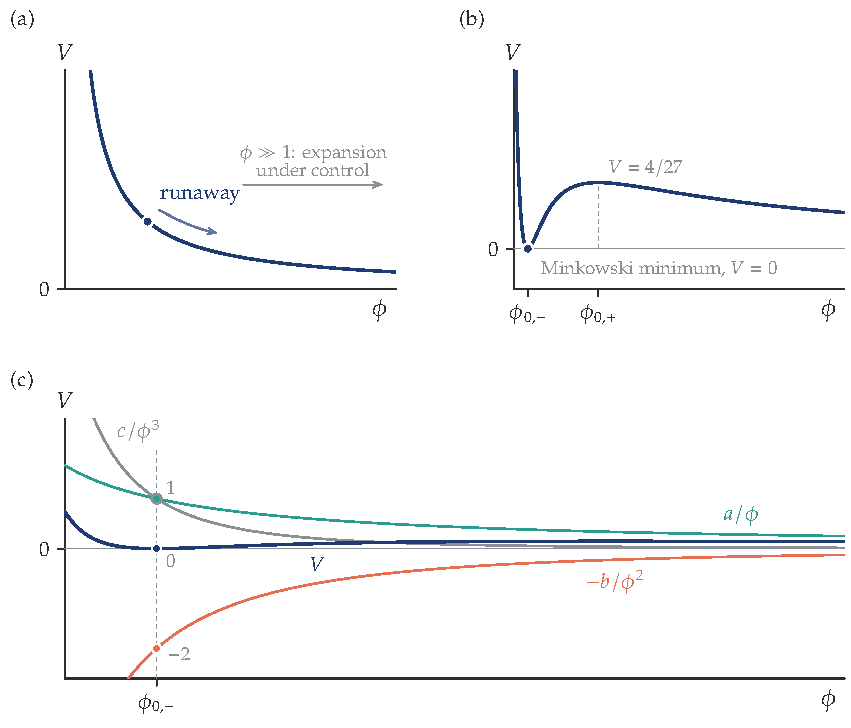
\includegraphics{fig_L3-dine-seiberg}
  \caption{The Dine--Seiberg problem in the toy model \cref{eq:L3-toy}. (a)~Where the expansion can be trusted, $\phi\gg1$, only the leading term survives, $V\simeq a/\phi$, and the modulus runs away to $\phi\to\infty$. (b)~Keeping three terms, with $ac = b^2/4$, gives a Minkowski minimum at $\phi_{0,-} = b/2a$ and a maximum at $\phi_{0,+} = 3b/2a$. (c)~At the minimum the three terms are of the same size, here $1$, $-2$ and $1$, and cancel.}\label{fig:L3-dine-seiberg}
\end{figure}

Can one then be in the limit $\phi\gg1$? With \cref{eq:L3-minkowski}, the expression \cref{eq:L3-roots} for the minimum becomes
\begin{equation}
  \phi_{0,-} = \frac{b}{2a}\gg1\qquad\text{if}\qquad b\gg a ,
  \qquad\text{and then}\qquad
  c = \frac{b^2}{4a}\gg b\gg a .
  \label{eq:L3-hierarchy}
\end{equation}
This contradicts \cref{eq:L3-natural}: one needs a hierarchy among the coefficients, $c\gg b\gg a$, which is a tuning. Is this natural? Is it even feasible? Moreover, the three contributions to the potential at the minimum are
\begin{equation}
  V(\phi_{0,-}) = \frac{a}{\phi_{0,-}} - \frac{b}{\phi_{0,-}^2} + \frac{c}{\phi_{0,-}^3}
  = \frac{2a^2}{b} - \frac{4a^2}{b} + \frac{2a^2}{b} = 0 .
  \label{eq:L3-terms}
\end{equation}
They cancel, but they are all of the same order, $a^2/b$. Why, then, should the term in $1/\phi^4$ be negligible? The only reason why one could still be at weak coupling, ignoring four loops, five loops and so on, is the tuning that makes $\phi$ big, $c\gg b\gg a$; but nothing guarantees that the same tuning does not also enhance the coefficient of $1/\phi^4$. Either one can trust the effective theory, and then there is no minimum, or one finds minima by balancing different terms of the same expansion, and then the result is always dirty. This is the \emph{Dine--Seiberg problem}, named after the paper that pointed it out~\cite{DineSeiberg}. It is not specific to the heterotic string, but a general problem of moduli stabilisation.

\subsection{The way out: balancing different expansions}
\label{sec:L3-way-out}

The Dine--Seiberg problem has been solved, by constructions found from the early 2000s onwards, which will be studied in equations towards the end of the course. The way out uses the fact that in string theory there is not just one expansion of the quantum corrections but three, the $g_s$, $\alpha'$ and non-perturbative expansions of \cref{eq:L3-Vquantum}. Each of them can be under control, with its first term much bigger than its second, and yet the first term of one expansion can balance the first term of another. A minimum found in this way can be fully under control. The idea is therefore to balance not different terms of the same expansion, but terms of different expansions: for example $\alpha'$ corrections against string-loop corrections, or perturbative against non-perturbative corrections. There are two famous solutions of this kind. One is \emph{KKLT}, from the initials of its authors, Kachru, Kallosh, Linde and Trivedi~\cite{KKLT}. The other, which appeared shortly afterwards, is the \emph{Large Volume Scenario} (LVS)~\cite{LVS}, in which, as the name says, the volume of the extra dimensions is very large.

\section{The cosmological moduli problem}
\label{sec:L3-CMP}

We now derive the bound \cref{eq:L3-CMP-bound}. There is no string theory in the argument, only the cosmology of a heavy scalar field with gravitational couplings, which must decay before Big Bang nucleosynthesis.

\subsection{A modulus displaced by inflation}

Suppose that the quantum corrections, in a scenario such as KKLT or the LVS, have produced a minimum in a regime in which the effective theory can be trusted, and shift the field so that the minimum is at zero. However complicated the potential is, around the minimum it is quadratic,
\begin{equation}
  V(\phi) = \frac12m_\phi^2\phi^2 \qquad\text{(at zero temperature)} ,
  \label{eq:L3-V0}
\end{equation}
where $\phi$ is now the canonically normalised modulus, of mass dimension one, and $m_\phi$ the mass of this spin-zero particle, which interacts gravitationally with everything.

In the very early universe, during inflation, the inflationary energy density, set by the Hubble rate as $\rho_{\text{inf}} = 3H^2\Mp^2$, contributes to the potential for the moduli, as any source of energy does, since the moduli couple gravitationally to it. A toy model of its effect is
\begin{equation}
  V(\phi) = \frac12m_\phi^2\phi^2 + \frac12H^2(\phi-\phi_0)^2
  \simeq \frac12H^2(\phi-\phi_0)^2 \qquad\text{for } H\gg m_\phi ,
  \label{eq:L3-Vinf}
\end{equation}
where the second term is the effect of inflation, with a coefficient of order one in general, here set to one. During inflation $H$ is much bigger than $m_\phi$: the inflationary Hubble scale can be as high as $10^{13}$--$10^{14}\GeV$ (present bounds on primordial gravitational waves require $H\lesssim5\times10^{13}\GeV$), while the modulus is much lighter. The minimum is then shifted to $\phi = H^2\phi_0/(H^2+m_\phi^2)\simeq\phi_0$, as in \cref{fig:L3-displacement}: in the early universe the field sits not at zero but at $\phi_0$. Since everything here is gravitational, the shift is expected to be of the order of the Planck scale, $\phi_0\sim\Mp$.

\begin{figure}[tbp]
  \centering
  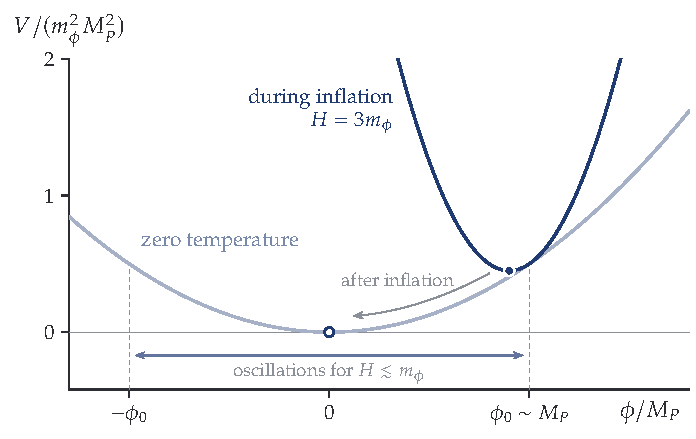
\includegraphics{fig_L3-displacement}
  \caption{A modulus during and after inflation. At zero temperature its potential is $\frac12m_\phi^2\phi^2$, with the minimum at $\phi = 0$ (light curve); during inflation the Hubble-induced term of \cref{eq:L3-Vinf}, with $H\gg m_\phi$ (here $H = 3m_\phi$), moves the minimum to $\phi\simeq\phi_0$ (dark curve). After inflation the field is left at $\phi_0$, far from the late-time minimum, and starts oscillating around it when $H\simeq m_\phi$.}\label{fig:L3-displacement}
\end{figure}

The evolution of the field is governed by the Klein--Gordon equation in an expanding universe, with the Friedmann--Lemaître--Robertson--Walker metric of the conventions. For a field that is homogeneous in space it reads
\begin{equation}
  \ddot\phi + 3H\dot\phi + m_\phi^2\phi = 0 .
  \label{eq:L3-KG}
\end{equation}
For $H = 0$ this is a harmonic oscillator. The term $3H\dot\phi$, due to the expansion of the universe, acts as friction, and for $H\gg m_\phi$ it dominates: the field is stuck at $\phi_0$, high up in the potential. As the universe expands, $H$ decreases, the potential approaches the zero-temperature one, \cref{eq:L3-V0}, and the friction becomes less and less important compared with the restoring force, until $H$ becomes of order $m_\phi$ and the field starts oscillating around the minimum:
\begin{equation}
  H_{\text{osc}}\simeq m_\phi .
  \label{eq:L3-Hosc}
\end{equation}
The initial amplitude is $\phi_0$, so the oscillations are large and the field stores energy instead of sitting at the minimum. While the field is stuck, its energy is only a small contribution to the vacuum energy; at the onset of the oscillations it is of the order of the potential,
\begin{equation}
  \rho_\phi^{\text{osc}}\simeq m_\phi^2\phi_0^2\simeq m_\phi^2\Mp^2 .
  \label{eq:L3-rho-phi}
\end{equation}

\subsection{Modulus domination and decay}

This energy density has to be compared with that of the standard cosmological history. After inflation the inflaton decays and reheats the universe: its energy goes into the particles of the Standard Model, which form a thermal bath and redshift as radiation. While the modulus is stuck it carries no energy density of its own, and all the energy is in radiation. But when $H$ drops to $m_\phi$, during radiation domination, part of the energy is in the oscillating $\phi$. The energy density of radiation at that time follows from the Friedmann equation, $3H^2\Mp^2 = \rho$:
\begin{equation}
  \rho_\gamma^{\text{osc}}\simeq H_{\text{osc}}^2\Mp^2\simeq m_\phi^2\Mp^2 .
  \label{eq:L3-rho-gamma}
\end{equation}
The two energy densities, \cref{eq:L3-rho-phi,eq:L3-rho-gamma}, are comparable: the modulus, which had no energy of its own, has as much energy as the whole Standard Model as soon as it starts oscillating.

As the universe expands both energy densities are diluted, but in different ways. A field oscillating coherently around its minimum is a condensate, a large number of quanta with zero momentum, and so it behaves as matter, which redshifts more slowly than radiation,
\begin{equation}
  \rho_\phi\propto a^{-3} ,\qquad \rho_\gamma\propto a^{-4} ,
  \label{eq:L3-redshift}
\end{equation}
where the scale factor $a$ grows with the expansion. Since the two start with comparable energies, $\phi$ very quickly comes to dominate the energy density of the universe.

This is the problem anticipated in \cref{sec:L3-requirements}. A stable modulus carries so much energy that it overcloses the universe, as too much dark matter. A modulus that decays into Standard Model particles converts all its energy into radiation, a huge injection of energy that dilutes all the particles present before, and with them the successful predictions for the abundances of the light elements. The decay happens when $H$ becomes of order the decay rate of $\phi$,
\begin{equation}
  H_{\text{dec}}\simeq\Gamma_{\phi\to\text{SM}} .
  \label{eq:L3-dec}
\end{equation}
since $1/H$ is the age of the universe and $1/\Gamma = \tau$ the lifetime of the particle. The history of the universe is then modified as in \cref{fig:L3-history}(a): after inflation and radiation domination comes an epoch of $\phi$ domination; when $\phi$ decays the universe returns to radiation domination, and then to matter and cosmological-constant domination as usual. Since everything produced before the decay is diluted, the decay must happen before Big Bang nucleosynthesis starts.

\begin{figure}[tbp]
  \centering
  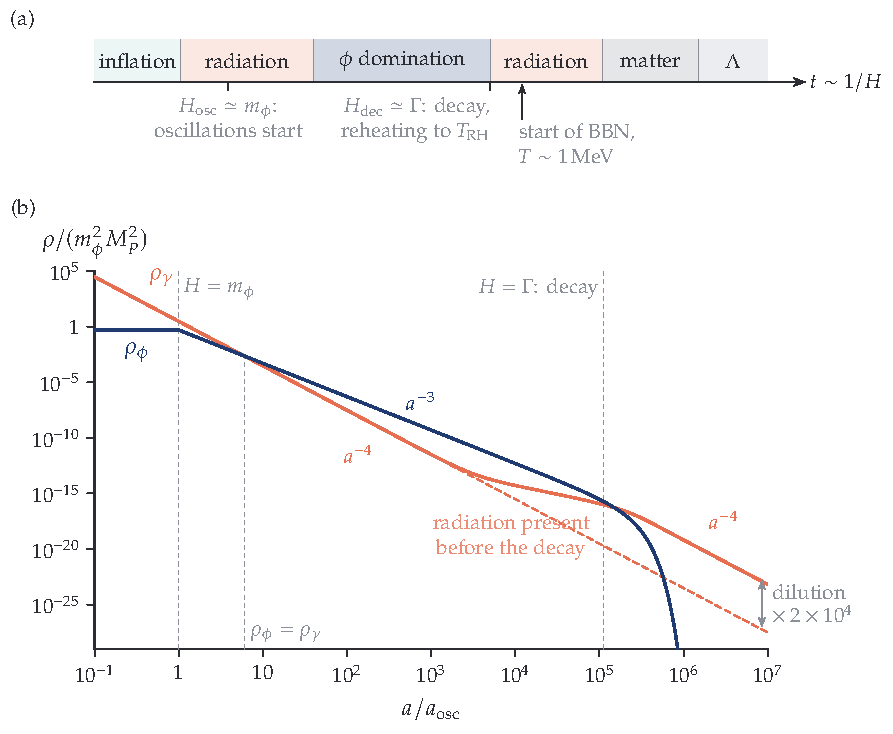
\includegraphics{fig_L3-history}
  \caption{Cosmological history with a displaced modulus. (a)~The sequence of epochs: inflation, radiation domination, domination by the oscillating modulus, radiation domination again after its decay, then matter and cosmological-constant domination. The modulus must decay before Big Bang nucleosynthesis starts. (b)~Energy densities of the modulus and of radiation as functions of the scale factor, from the onset of the oscillations at $H_{\text{osc}}\simeq m_\phi$ to the decay at $H_{\text{dec}}\simeq\Gamma$; the dashed line is the radiation present before the decay, diluted by it. The ratio $\Gamma/m_\phi = 10^{-8}$ is chosen for illustration; for a real modulus it is $(m_\phi/\Mp)^2\sim10^{-28}$.}\label{fig:L3-history}
\end{figure}

\subsection{The bound on the mass of the moduli}

To estimate $\Gamma_{\phi\to\text{SM}}$, note that the moduli couple to the gauge bosons: the gauge kinetic function, a function of the fields as seen in the supersymmetry course, depends in string compactifications on the moduli. Expanding it around the minimum gives a coupling of $\phi$ to two gauge bosons, suppressed by the Planck mass,
\begin{equation}
  \mathcal L_4\supset\frac{\phi}{\Mp}\,F_{\mu\nu}F^{\mu\nu} ,
  \label{eq:L3-phiFF}
\end{equation}
up to a coefficient of order one, through which the modulus decays as in \cref{fig:L3-decay}, very weakly. Dimensional analysis is enough to estimate the rate. It goes like the square of the coupling, $1/\Mp^2$, and has dimensions of a mass, so it must contain a mass cubed, and the only mass available in the decay into massless gauge bosons is $m_\phi$:
\begin{equation}
  \Gamma_{\phi\to\text{SM}}\simeq\frac{m_\phi^3}{\Mp^2} .
  \label{eq:L3-Gamma}
\end{equation}

\begin{figure}[tbp]
  \centering
  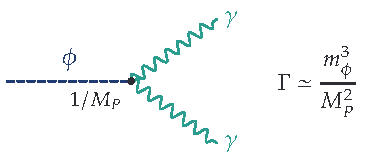
\includegraphics{fig_L3-decay}
  \caption{Decay of a modulus into two gauge bosons through the coupling \cref{eq:L3-phiFF}, with one vertex suppressed by $1/\Mp$, which gives $\Gamma\simeq m_\phi^3/\Mp^2$ (\cref{eq:L3-Gamma}).}\label{fig:L3-decay}
\end{figure}

The Hubble rate at the decay is then
\begin{equation}
  H_{\text{dec}}\simeq\Gamma_{\phi\to\text{SM}}\simeq m_\phi\Bigl(\frac{m_\phi}{\Mp}\Bigr)^2
  \simeq H_{\text{osc}}\Bigl(\frac{m_\phi}{\Mp}\Bigr)^2\ll H_{\text{osc}} ,
  \label{eq:L3-Hdec}
\end{equation}
by \cref{eq:L3-Hosc}, since the moduli are much lighter than the Planck scale: the moduli decay long after they start oscillating.

The decay reheats the universe, and $H_{\text{dec}}$ is the Hubble rate at the start of the new epoch of radiation domination, $H\simeq T^2/\Mp$ (see the conventions), at a temperature called the \emph{reheating temperature} $T_{\text{RH}}$. Hence
\begin{equation}
  H_{\text{dec}}\simeq\Gamma_{\phi\to\text{SM}}\simeq\frac{T_{\text{RH}}^2}{\Mp}
  \qquad\Longrightarrow\qquad
  T_{\text{RH}}\simeq\sqrt{\Gamma_{\phi\to\text{SM}}\Mp}\simeq m_\phi\sqrt{\frac{m_\phi}{\Mp}} ,
  \label{eq:L3-TRH}
\end{equation}
where the last step uses \cref{eq:L3-Gamma}.

For the decay to happen before Big Bang nucleosynthesis, the reheating temperature must exceed the temperature at which the light elements started to form, of order one MeV:
\begin{equation}
  T_{\text{RH}} > T_{\text{BBN}}\sim1\,\mathrm{MeV}\sim10^{-21}\Mp .
  \label{eq:L3-TBBN}
\end{equation}
With \cref{eq:L3-TRH} this gives $m_\phi^{3/2}\gtrsim10^{-21}\Mp^{3/2}$, i.e.
\begin{equation}
  m_\phi\gtrsim10^{-14}\Mp\sim10^4\GeV ,
  \label{eq:L3-mass-bound}
\end{equation}
a mass of order $10\TeV$. A more precise computation, keeping all the factors dropped in the signs $\simeq$, gives $30\TeV$: this is where the bound \cref{eq:L3-CMP-bound} comes from.

String compactifications must therefore make the moduli quite heavy. The bound can be evaded if the cosmological history has new features. The estimate assumed an initial displacement $\phi_0$ of order $\Mp$; if some mechanism made it much smaller, the energy stored in $\phi$ and the dilution would be much smaller too, and the cosmological history would have to be studied in detail. Alternatively, the displacement could be of order $\Mp$ but the moduli themselves diluted by something else in some epoch. So the bound \cref{eq:L3-CMP-bound} is much stronger than the bound \cref{eq:L2-bound} from fifth forces, and generically present, but it depends somewhat on the cosmology, whereas the much weaker one from fifth forces rests on observations made today.

In the next lecture we start looking at type IIB in equations: first D-branes and their effective action, then the bulk action, and how Calabi--Yau manifolds emerge.


\renewcommand{\bibname}{References}
\begin{thebibliography}{99}
\addcontentsline{toc}{chapter}{References}

\bibitem{IbanezUranga}
L.~E. Ibáñez and A.~M. Uranga, \emph{String Theory and Particle Physics: An Introduction to String Phenomenology}, Cambridge University Press, 2012.

\bibitem{Hebecker}
A.~Hebecker, \emph{Naturalness, String Landscape and Multiverse}, Lecture Notes in Physics 979, Springer, 2021, \texttt{arXiv:2008.10625}.

\bibitem{BKLS}
R.~Blumenhagen, B.~Körs, D.~Lüst and S.~Stieberger, \emph{Four-dimensional string compactifications with D-branes, orientifolds and fluxes}, Phys.\ Rept.\ \textbf{445} (2007) 1, \texttt{hep-th/0610327}.

\bibitem{Louis}
J.~Louis, lecture notes on string theory and string compactifications, available on the author's website (University of Hamburg).

\bibitem{BaumannMcAllister}
D.~Baumann and L.~McAllister, \emph{Inflation and String Theory}, Cambridge University Press, 2015, \texttt{arXiv:1404.2601}.

\bibitem{StringCosmoReview}
M.~Cicoli, J.~P. Conlon, A.~Maharana, S.~Parameswaran, F.~Quevedo and I.~Zavala, \emph{String cosmology: from the early universe to today}, \texttt{arXiv:2303.04819}.

\bibitem{Polchinski}
J.~Polchinski, \emph{String Theory}, Vols.~I and~II, Cambridge University Press, 1998.

\bibitem{Tong}
D.~Tong, \emph{Lectures on String Theory}, \texttt{arXiv:0908.0333}.

\bibitem{CHSW}
P.~Candelas, G.~T. Horowitz, A.~Strominger and E.~Witten, \emph{Vacuum configurations for superstrings}, Nucl.\ Phys.\ B \textbf{258} (1985) 46.

\bibitem{BBHL}
K.~Becker, M.~Becker, M.~Haack and J.~Louis, \emph{Supersymmetry breaking and $\alpha'$-corrections to flux induced potentials}, JHEP \textbf{06} (2002) 060, \texttt{hep-th/0204254}.

\bibitem{GrimmLouis}
T.~W. Grimm and J.~Louis, \emph{The effective action of type IIB Calabi--Yau orientifolds}, Nucl.\ Phys.\ B \textbf{699} (2004) 387, \texttt{hep-th/0403067}.

\bibitem{KreuzerSkarke}
M.~Kreuzer and H.~Skarke, \emph{Complete classification of reflexive polyhedra in four dimensions}, Adv.\ Theor.\ Math.\ Phys.\ \textbf{4} (2000) 1209, \texttt{hep-th/0002240}.

\bibitem{Planck2018}
Planck Collaboration, N.~Aghanim et al., \emph{Planck 2018 results. VI. Cosmological parameters}, Astron.\ Astrophys.\ \textbf{641} (2020) A6, \texttt{arXiv:1807.06209}.

\bibitem{EotWash}
J.~G. Lee, E.~G. Adelberger, T.~S. Cook, S.~M. Fleischer and B.~R. Heckel, \emph{New test of the gravitational $1/r^2$ law at separations down to $52\,\mu$m}, Phys.\ Rev.\ Lett.\ \textbf{124} (2020) 101101, \texttt{arXiv:2002.11761}.

\bibitem{GKP}
S.~B. Giddings, S.~Kachru and J.~Polchinski, \emph{Hierarchies from fluxes in string compactifications}, Phys.\ Rev.\ D \textbf{66} (2002) 106006, \texttt{hep-th/0105097}.

\bibitem{GVW}
S.~Gukov, C.~Vafa and E.~Witten, \emph{CFT's from Calabi--Yau four-folds}, Nucl.\ Phys.\ B \textbf{584} (2000) 69, \texttt{hep-th/9906070}.

\bibitem{Strominger}
A.~Strominger, \emph{Superstrings with torsion}, Nucl.\ Phys.\ B \textbf{274} (1986) 253.

\bibitem{DineSeiberg}
M.~Dine and N.~Seiberg, \emph{Is the superstring weakly coupled?}, Phys.\ Lett.\ B \textbf{162} (1985) 299.

\bibitem{KKLT}
S.~Kachru, R.~Kallosh, A.~Linde and S.~P. Trivedi, \emph{De Sitter vacua in string theory}, Phys.\ Rev.\ D \textbf{68} (2003) 046005, \texttt{hep-th/0301240}.

\bibitem{LVS}
V.~Balasubramanian, P.~Berglund, J.~P. Conlon and F.~Quevedo, \emph{Systematics of moduli stabilisation in Calabi--Yau flux compactifications}, JHEP \textbf{03} (2005) 007, \texttt{hep-th/0502058}.

\bibitem{Coughlan}
G.~D. Coughlan, W.~Fischler, E.~W. Kolb, S.~Raby and G.~G. Ross, \emph{Cosmological problems for the Polonyi potential}, Phys.\ Lett.\ B \textbf{131} (1983) 59.

\bibitem{deCarlos}
B.~de Carlos, J.~A. Casas, F.~Quevedo and E.~Roulet, \emph{Model-independent properties and cosmological implications of the dilaton and moduli sectors of 4d strings}, Phys.\ Lett.\ B \textbf{318} (1993) 447, \texttt{hep-ph/9308325}.

\bibitem{BanksKaplanNelson}
T.~Banks, D.~B. Kaplan and A.~E. Nelson, \emph{Cosmological implications of dynamical supersymmetry breaking}, Phys.\ Rev.\ D \textbf{49} (1994) 779, \texttt{hep-ph/9308292}.

\bibitem{deSalas}
P.~F. de Salas, M.~Lattanzi, G.~Mangano, G.~Miele, S.~Pastor and O.~Pisanti, \emph{Bounds on very low reheating scenarios after Planck}, Phys.\ Rev.\ D \textbf{92} (2015) 123534, \texttt{arXiv:1511.00672}.

\end{thebibliography}

\end{document}
